%%%%%%%%%%%%%%%%%%%%%%%%%%%%%%%%%%%%%%%%%%%%%%%%%%%%%%%%%%%%%
\chapter{Remaining Spectral Models}\label{sec:pdx_spec_mdls}
%%%%%%%%%%%%%%%%%%%%%%%%%%%%%%%%%%%%%%%%%%%%%%%%%%%%%%%%%%%%%

\begin{figure}[h]
    \centering{
    \begin{tabular}{ccc}
        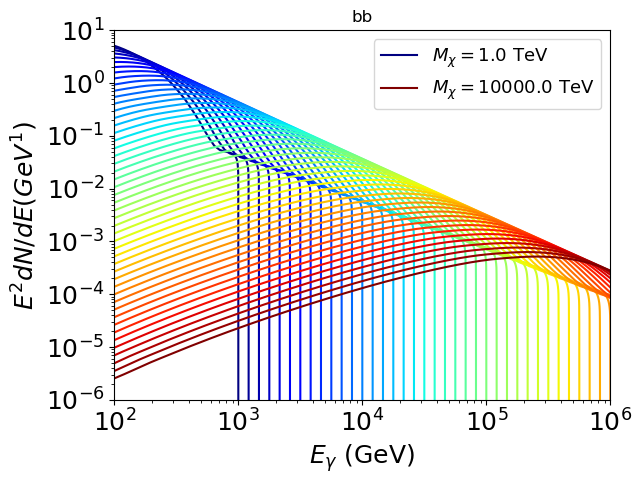
\includegraphics[scale=0.27]{figures/mtd_hawc_dm/hdm_bb.png} &
        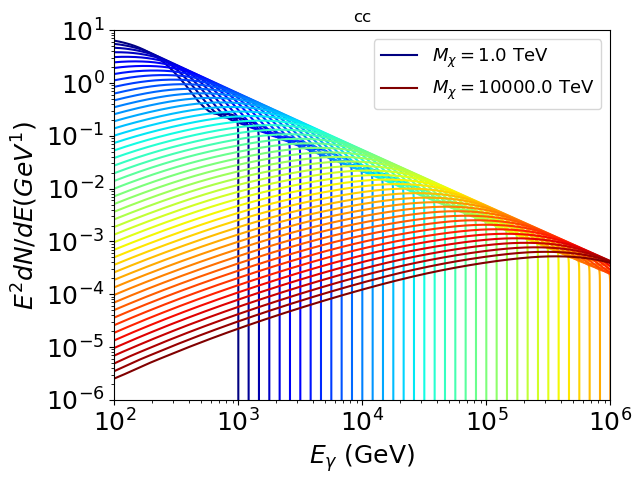
\includegraphics[scale=0.27]{figures/mtd_hawc_dm/hdm_cc.png} &
        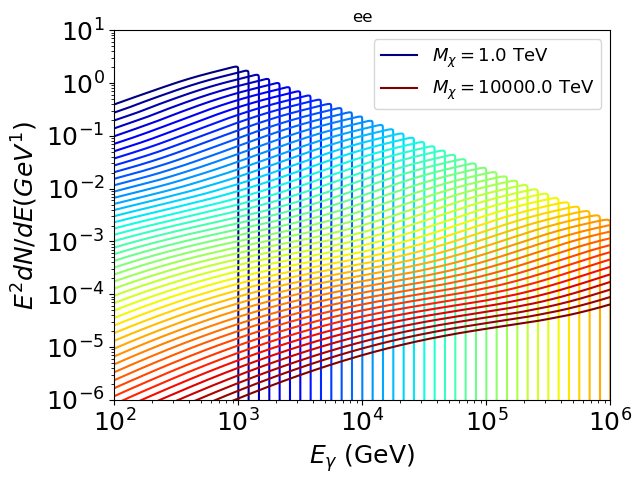
\includegraphics[scale=0.27]{figures/mtd_hawc_dm/hdm_ee.png} \\
        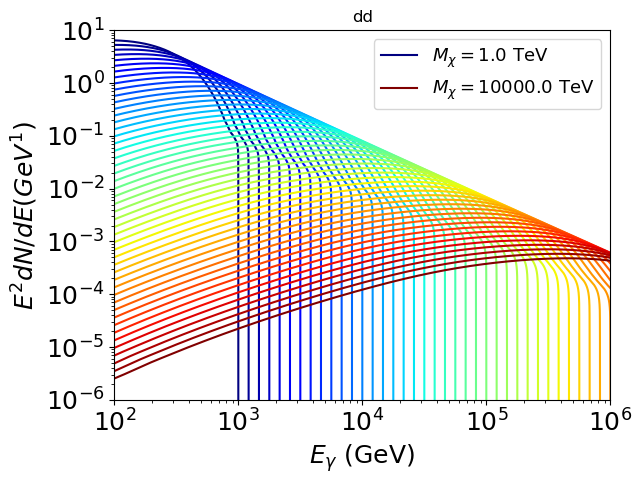
\includegraphics[scale=0.27]{figures/mtd_hawc_dm/hdm_dd.png} &
        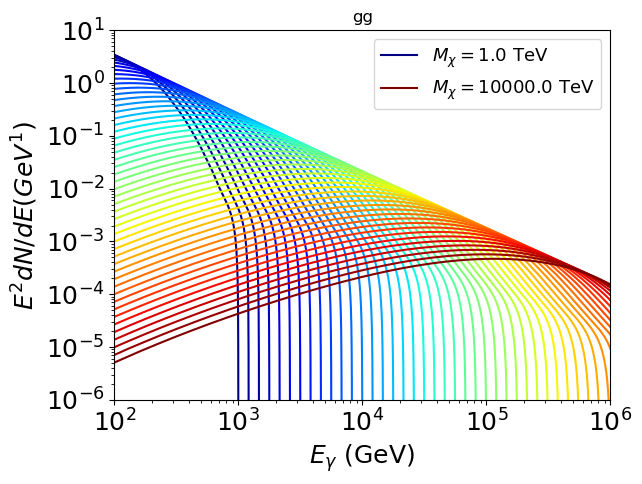
\includegraphics[scale=0.27]{figures/mtd_hawc_dm/hdm_gg.png} &
        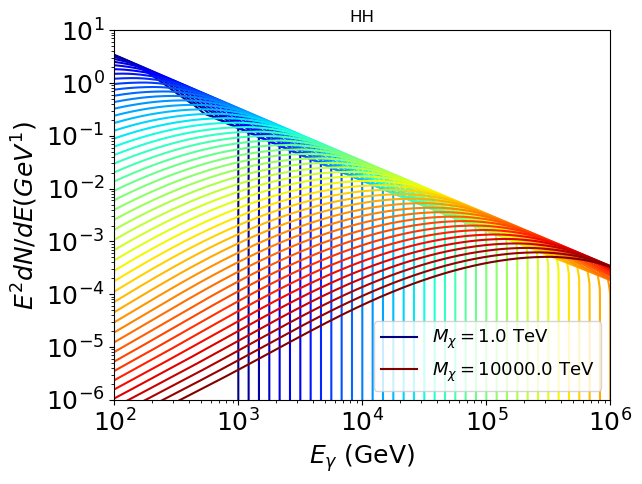
\includegraphics[scale=0.27]{figures/mtd_hawc_dm/hdm_hh.png} \\
        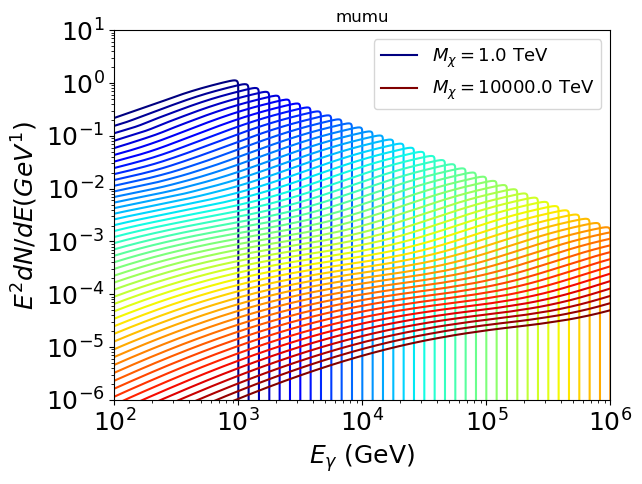
\includegraphics[scale=0.27]{figures/mtd_hawc_dm/hdm_mumu.png} &
        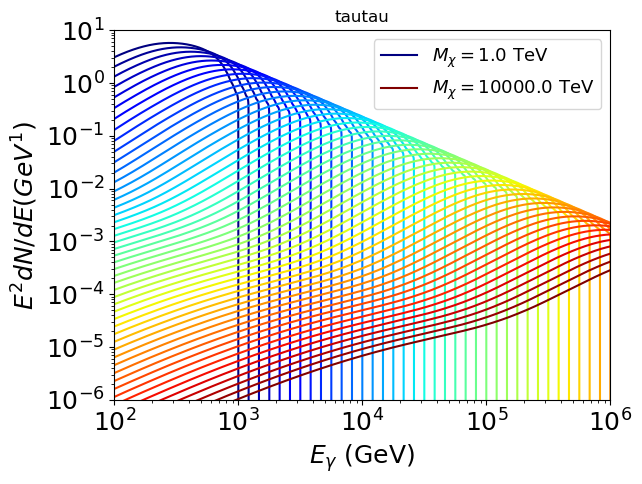
\includegraphics[scale=0.27]{figures/mtd_hawc_dm/hdm_tautau.png} &
        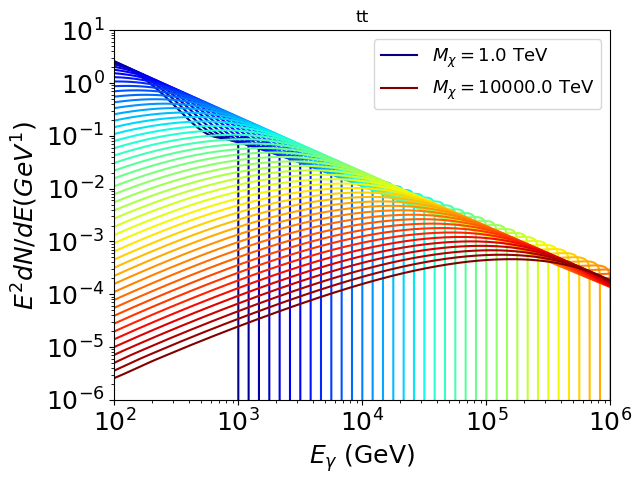
\includegraphics[scale=0.27]{figures/mtd_hawc_dm/hdm_tt.png} \\
        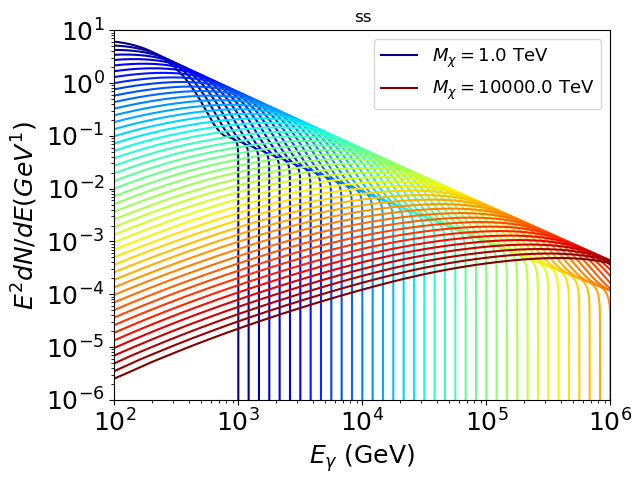
\includegraphics[scale=0.27]{figures/mtd_hawc_dm/hdm_ss.png} &
        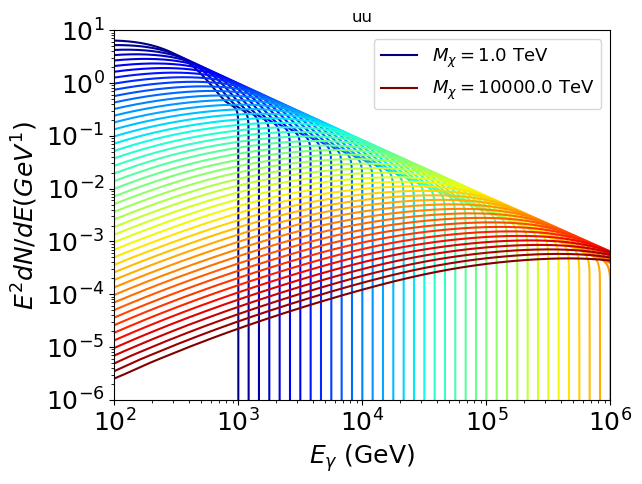
\includegraphics[scale=0.27]{figures/mtd_hawc_dm/hdm_uu.png} &
        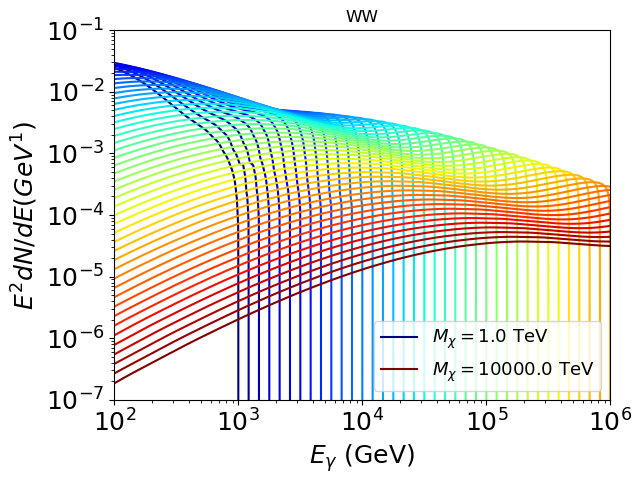
\includegraphics[scale=0.27]{figures/mtd_hawc_dm/hdm_ww.png} \\
        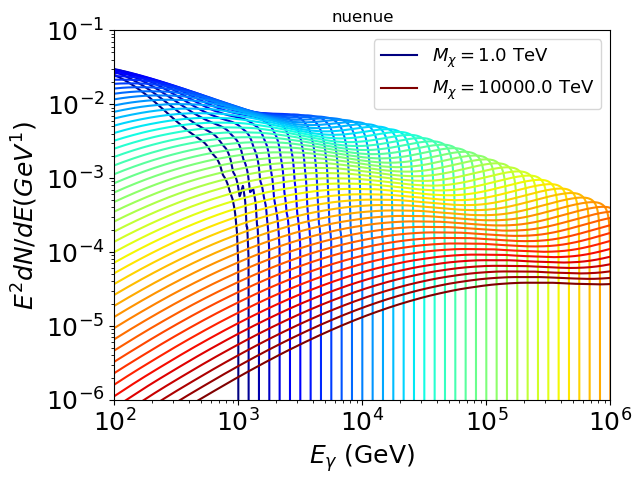
\includegraphics[scale=0.27]{figures/mtd_hawc_dm/hdm_nuenue.png} &
        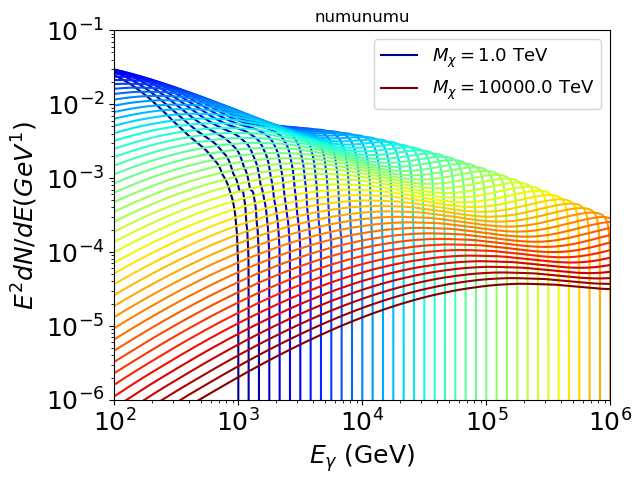
\includegraphics[scale=0.27]{figures/mtd_hawc_dm/hdm_numunumu.png} &
        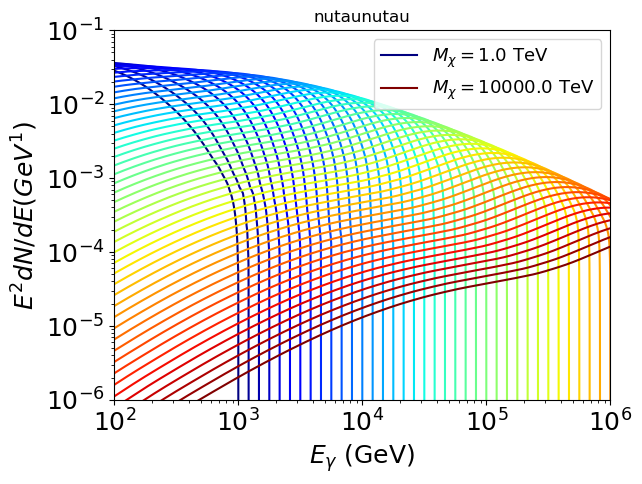
\includegraphics[scale=0.27]{figures/mtd_hawc_dm/hdm_nutaunutau.png} \\
    \end{tabular}
    }\caption{Sister figure to \Cref{fig:hdm_gamma_lines} for remaining SM primary annihilation channels studied for this thesis. These did not require any post generation smoothing and so are directly pulled from \cite{Rodd:HDM_spec} with a binning scheme most helpful for a HAWC analysis.
    }\label{fig:apdx_mtd_spectra}
\end{figure}

\clearpage
%%%%%%%%%%%%%%%%%%%%%%%%%%%%%%%%%%%%%%%%%%%%%%%%%%%%%%%%%%%%%
\chapter{mpu\_analysis.py}\label{sec:apx_mpu_script}
%%%%%%%%%%%%%%%%%%%%%%%%%%%%%%%%%%%%%%%%%%%%%%%%%%%%%%%%%%%%%

\lstinputlisting[language=Python]{appendices/mpu_analysis.py}
\clearpage

%%%%%%%%%%%%%%%%%%%%%%%%%%%%%%%%%%%%%%%%%%%%%%%%%%%%%%%%%%%%%
\chapter{Comparison with Glory Duck}\label{sec:apx_gd_vs_mtd}
%%%%%%%%%%%%%%%%%%%%%%%%%%%%%%%%%%%%%%%%%%%%%%%%%%%%%%%%%%%%%

\begin{figure}[h]
\centering{
    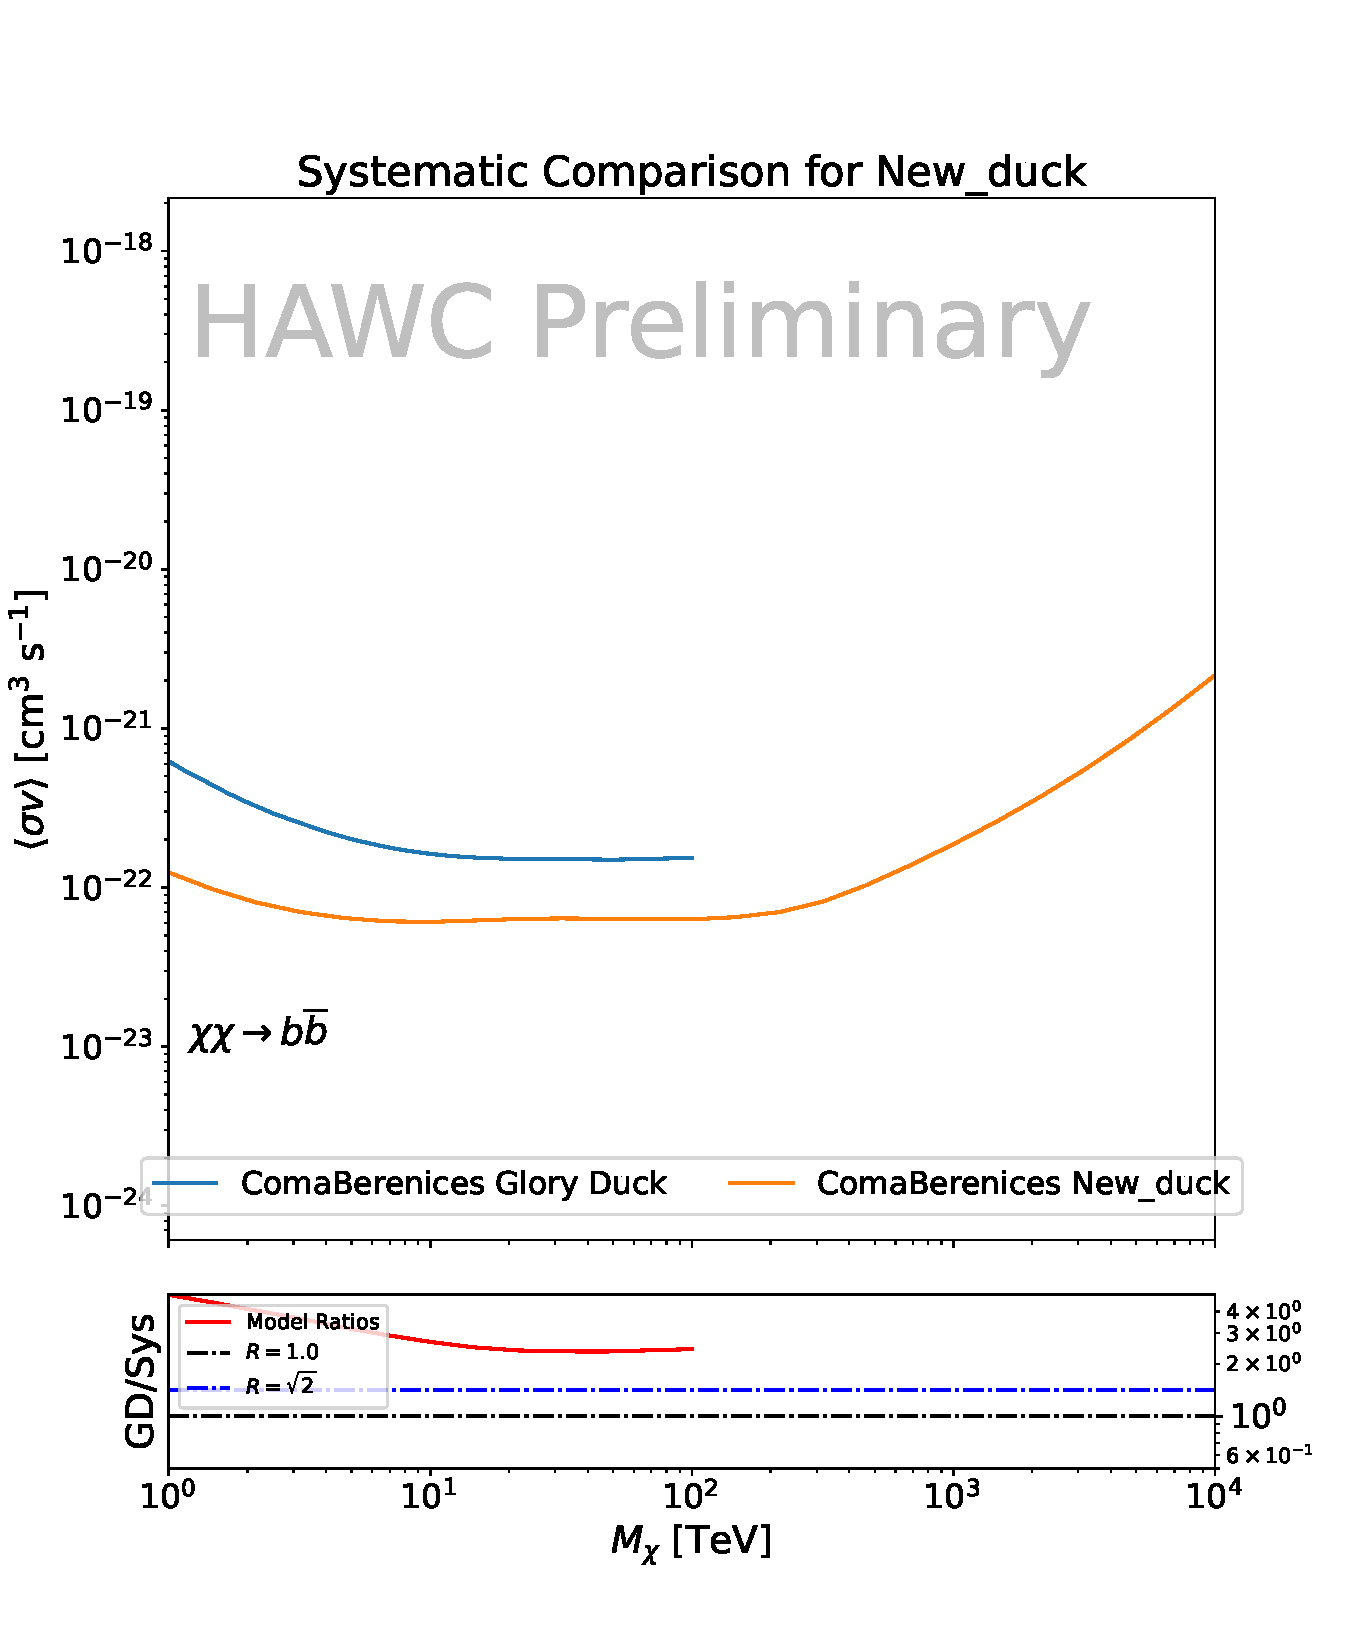
\includegraphics[scale=0.2]{figures/mtd_hawc_dm/systematics/Systematic_GD_New_duck_ComaBerenices_bb.pdf}
    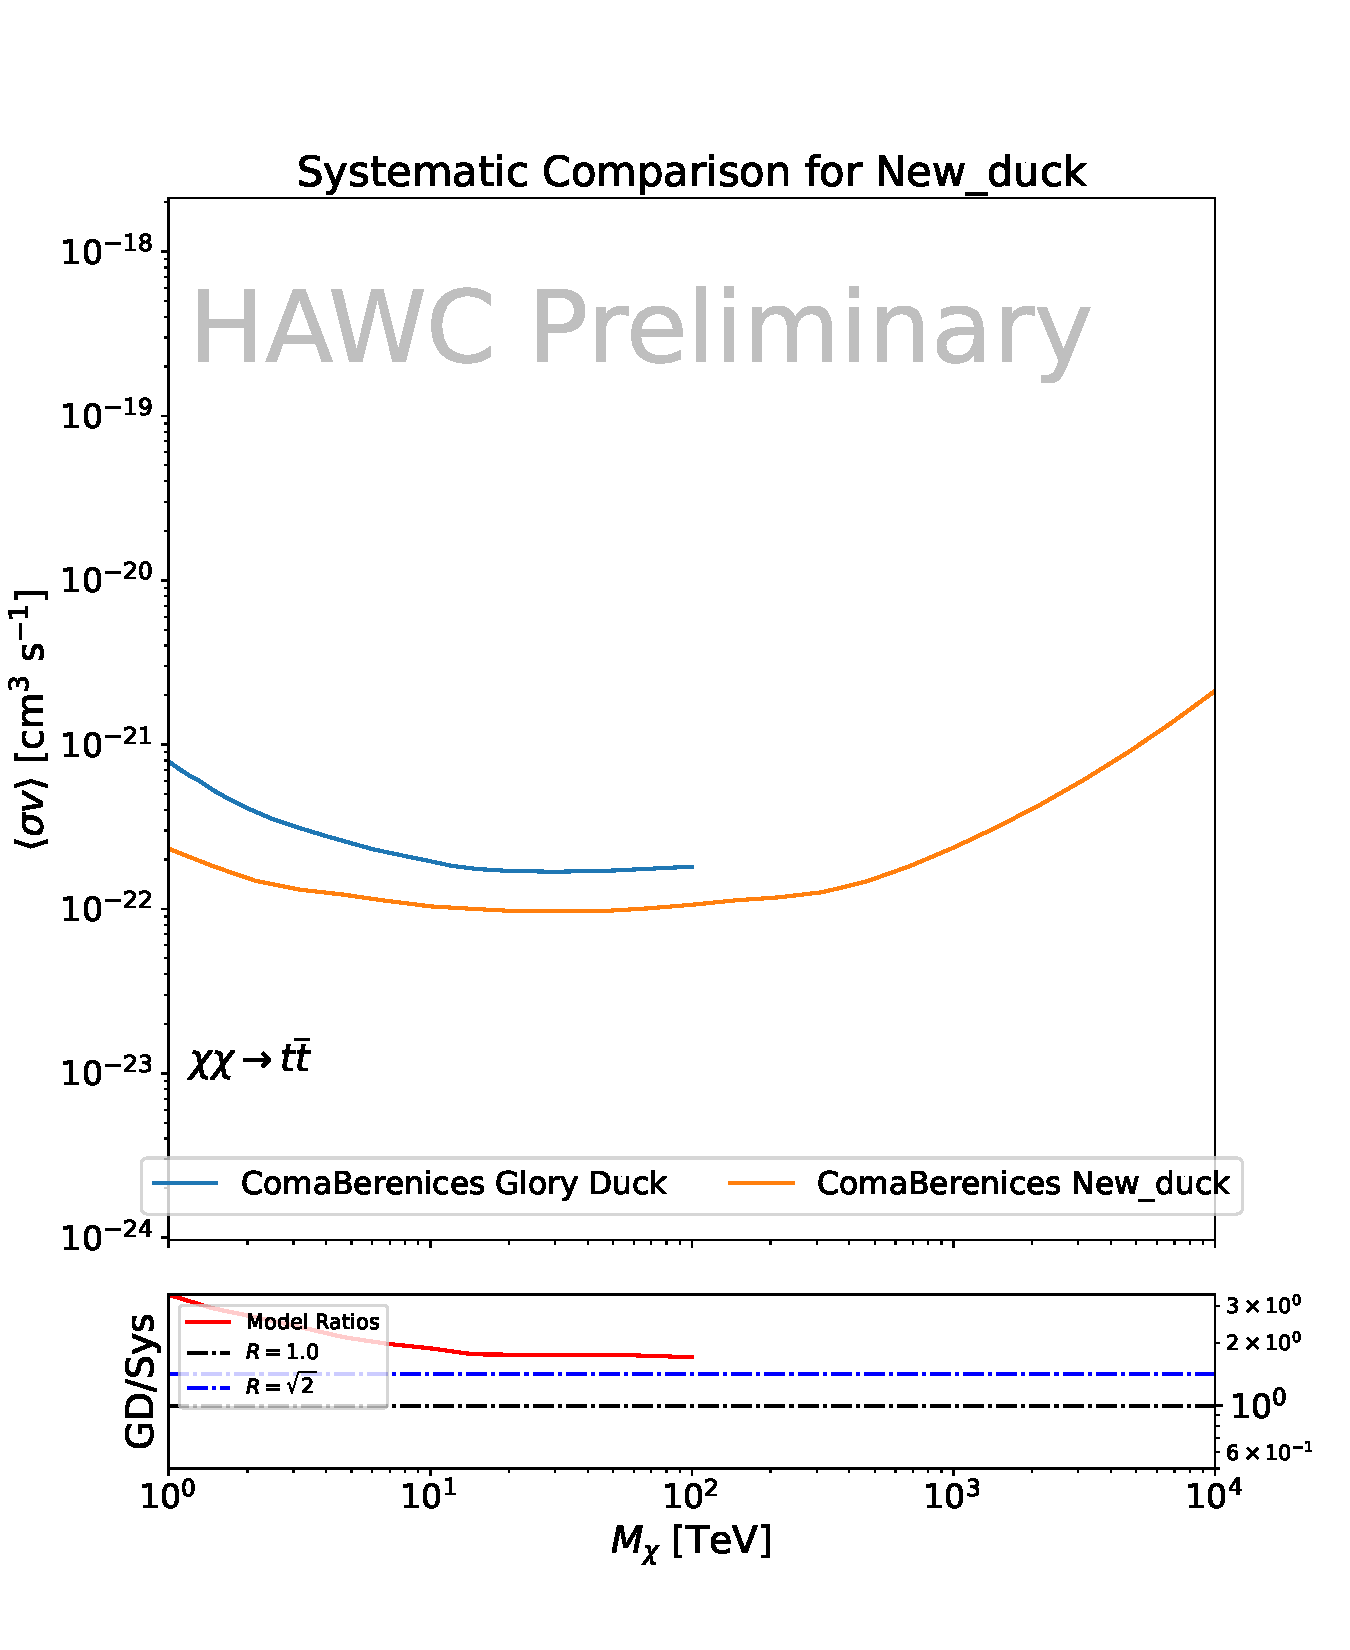
\includegraphics[scale=0.2]{figures/mtd_hawc_dm/systematics/Systematic_GD_New_duck_ComaBerenices_tt.pdf}
    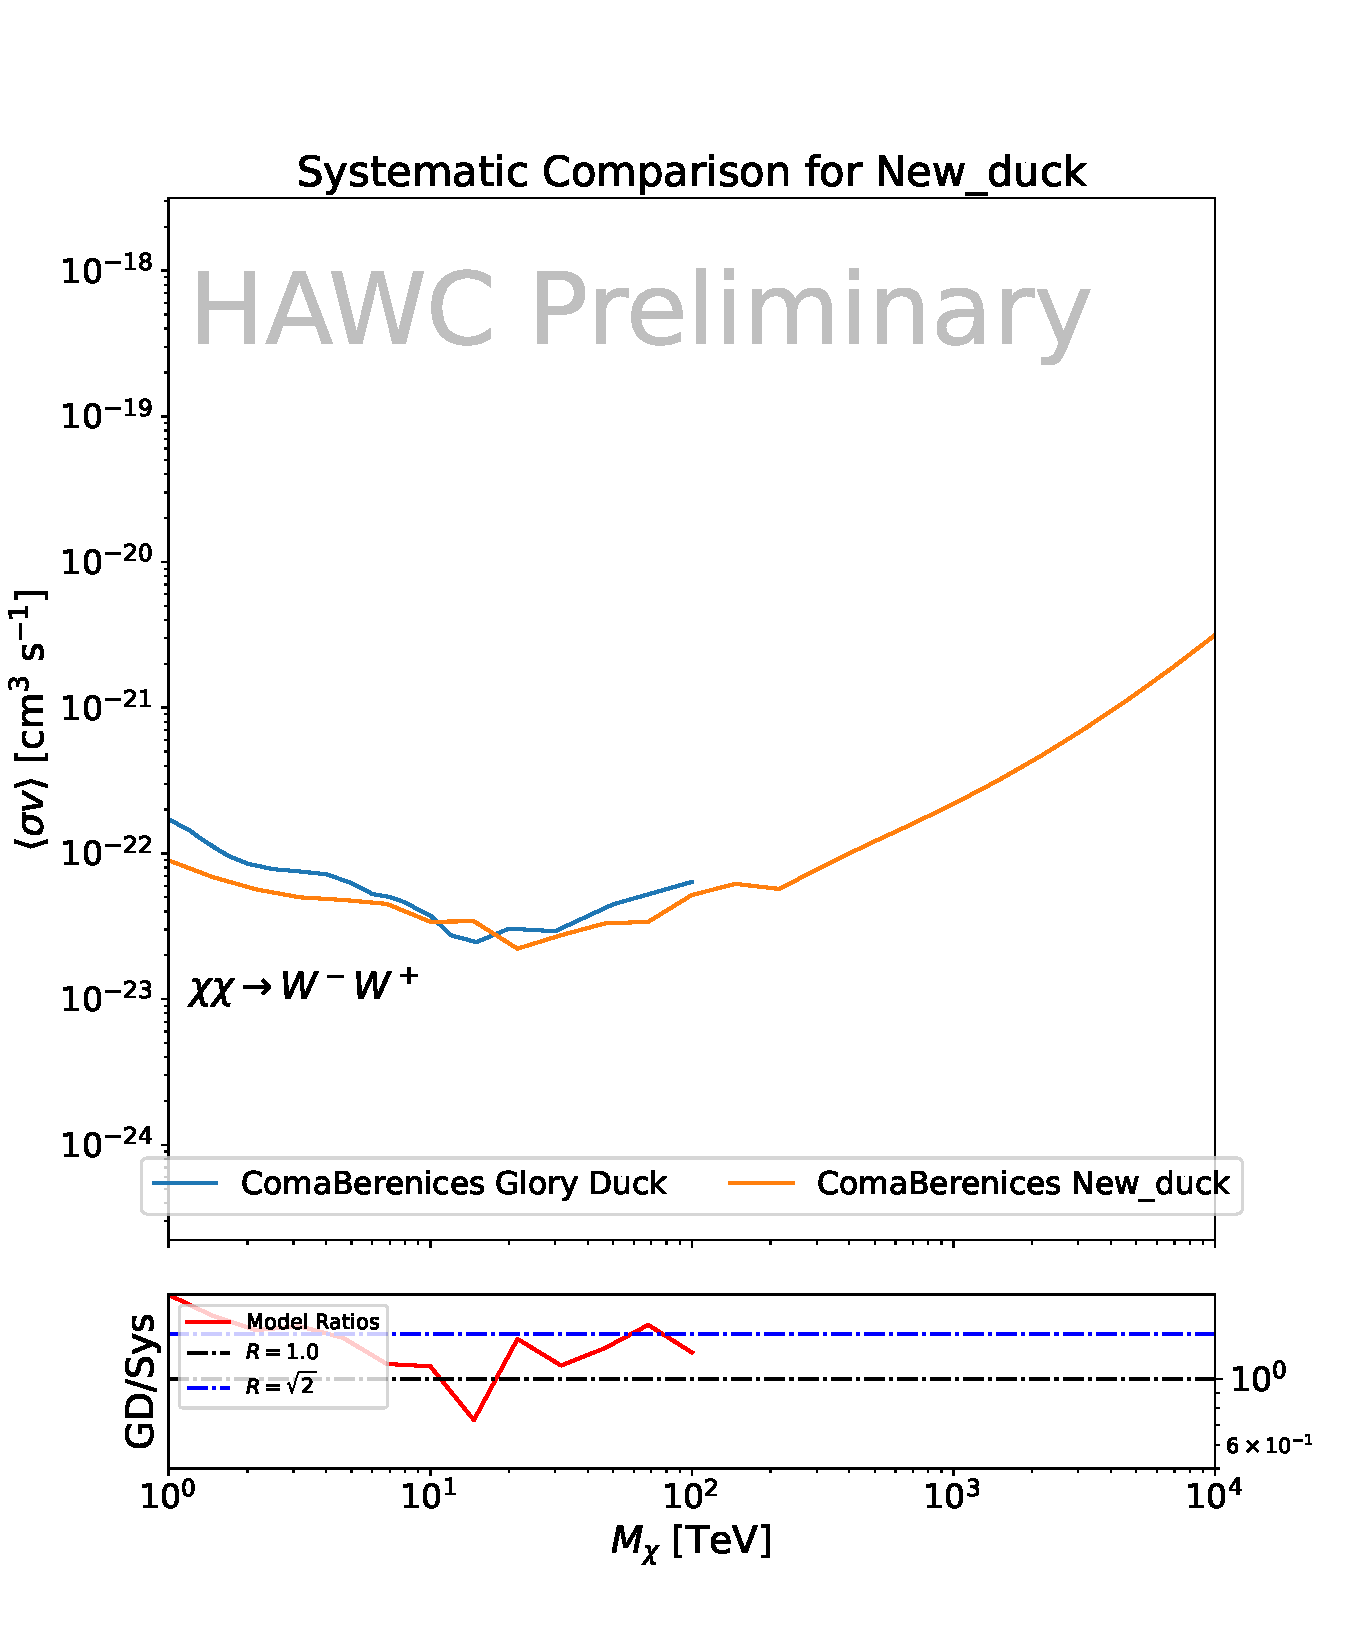
\includegraphics[scale=0.2]{figures/mtd_hawc_dm/systematics/Systematic_GD_New_duck_ComaBerenices_ww.pdf}
    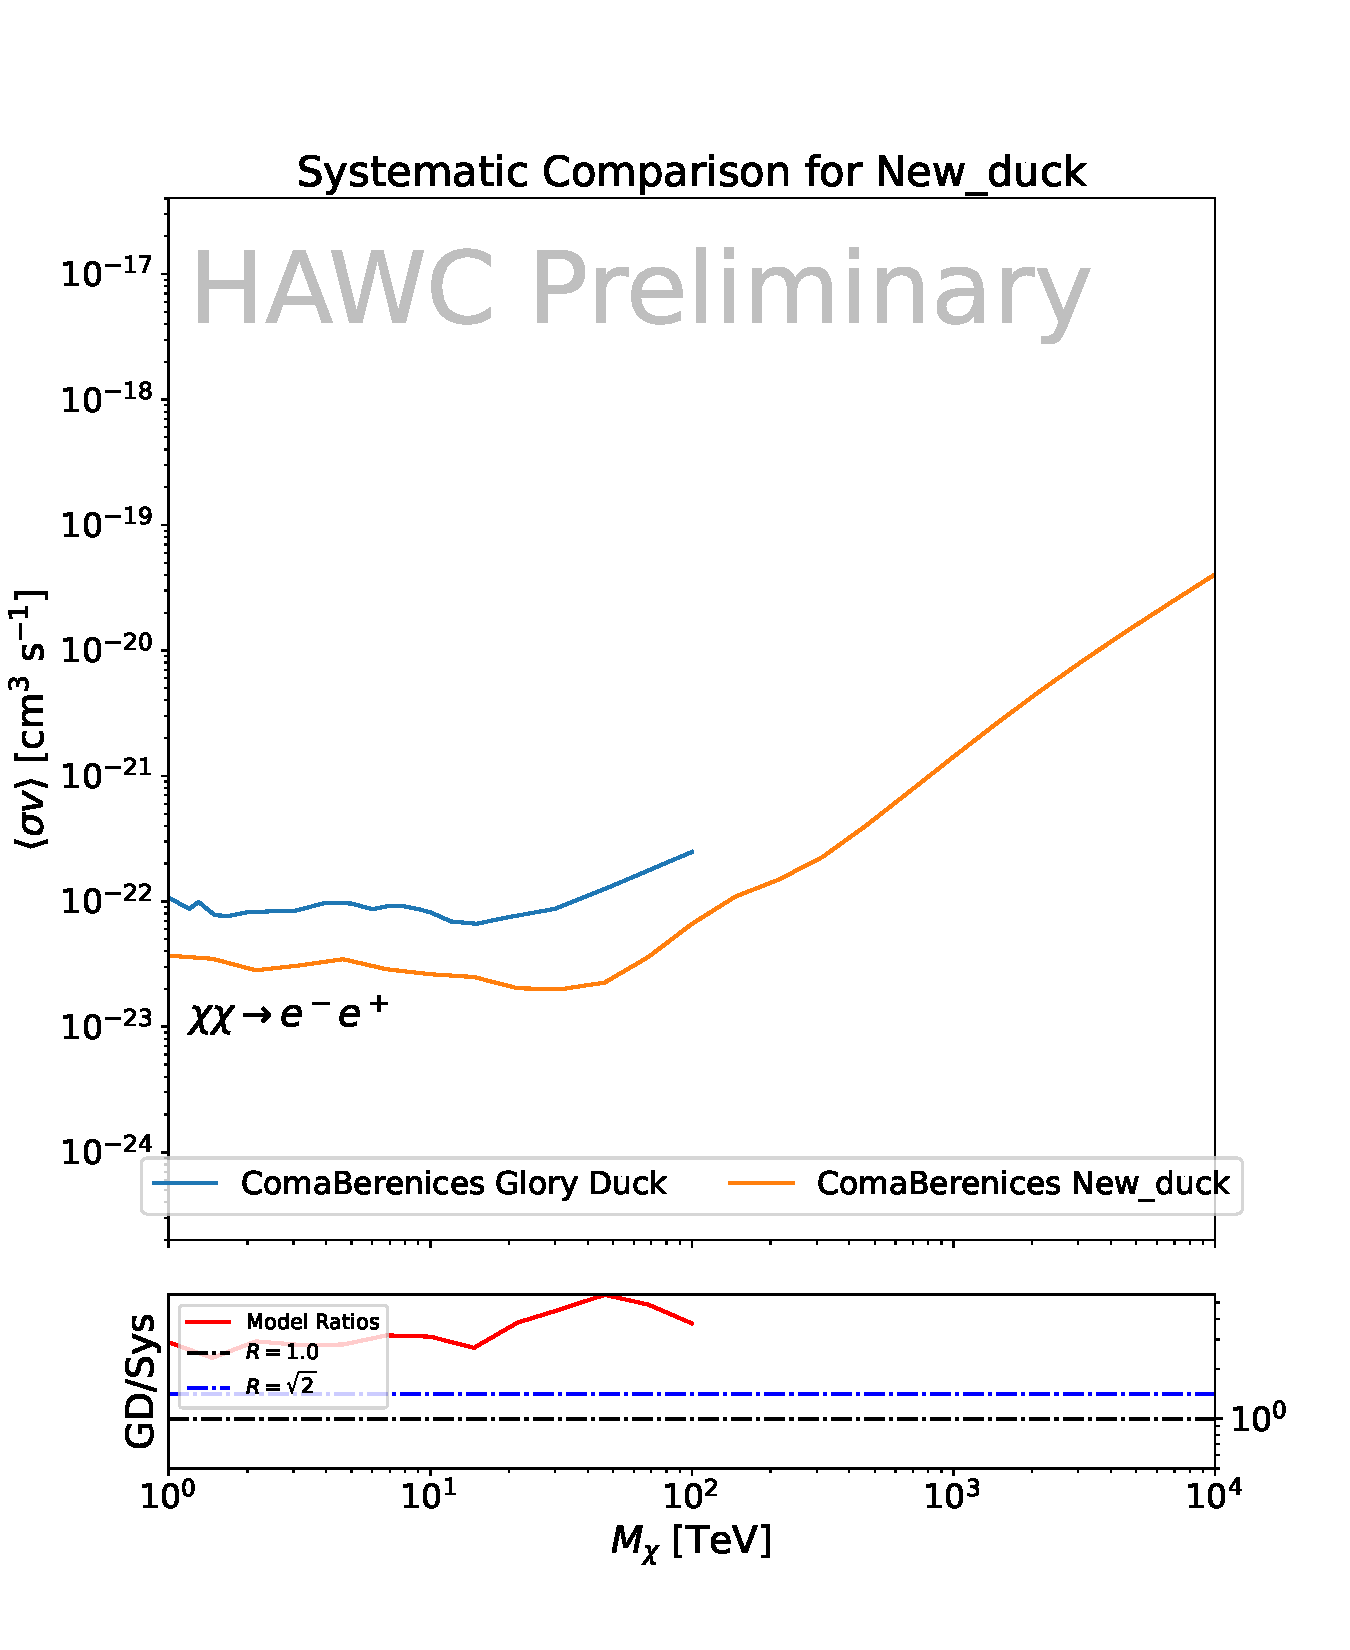
\includegraphics[scale=0.2]{figures/mtd_hawc_dm/systematics/Systematic_GD_New_duck_ComaBerenices_ee.pdf}
    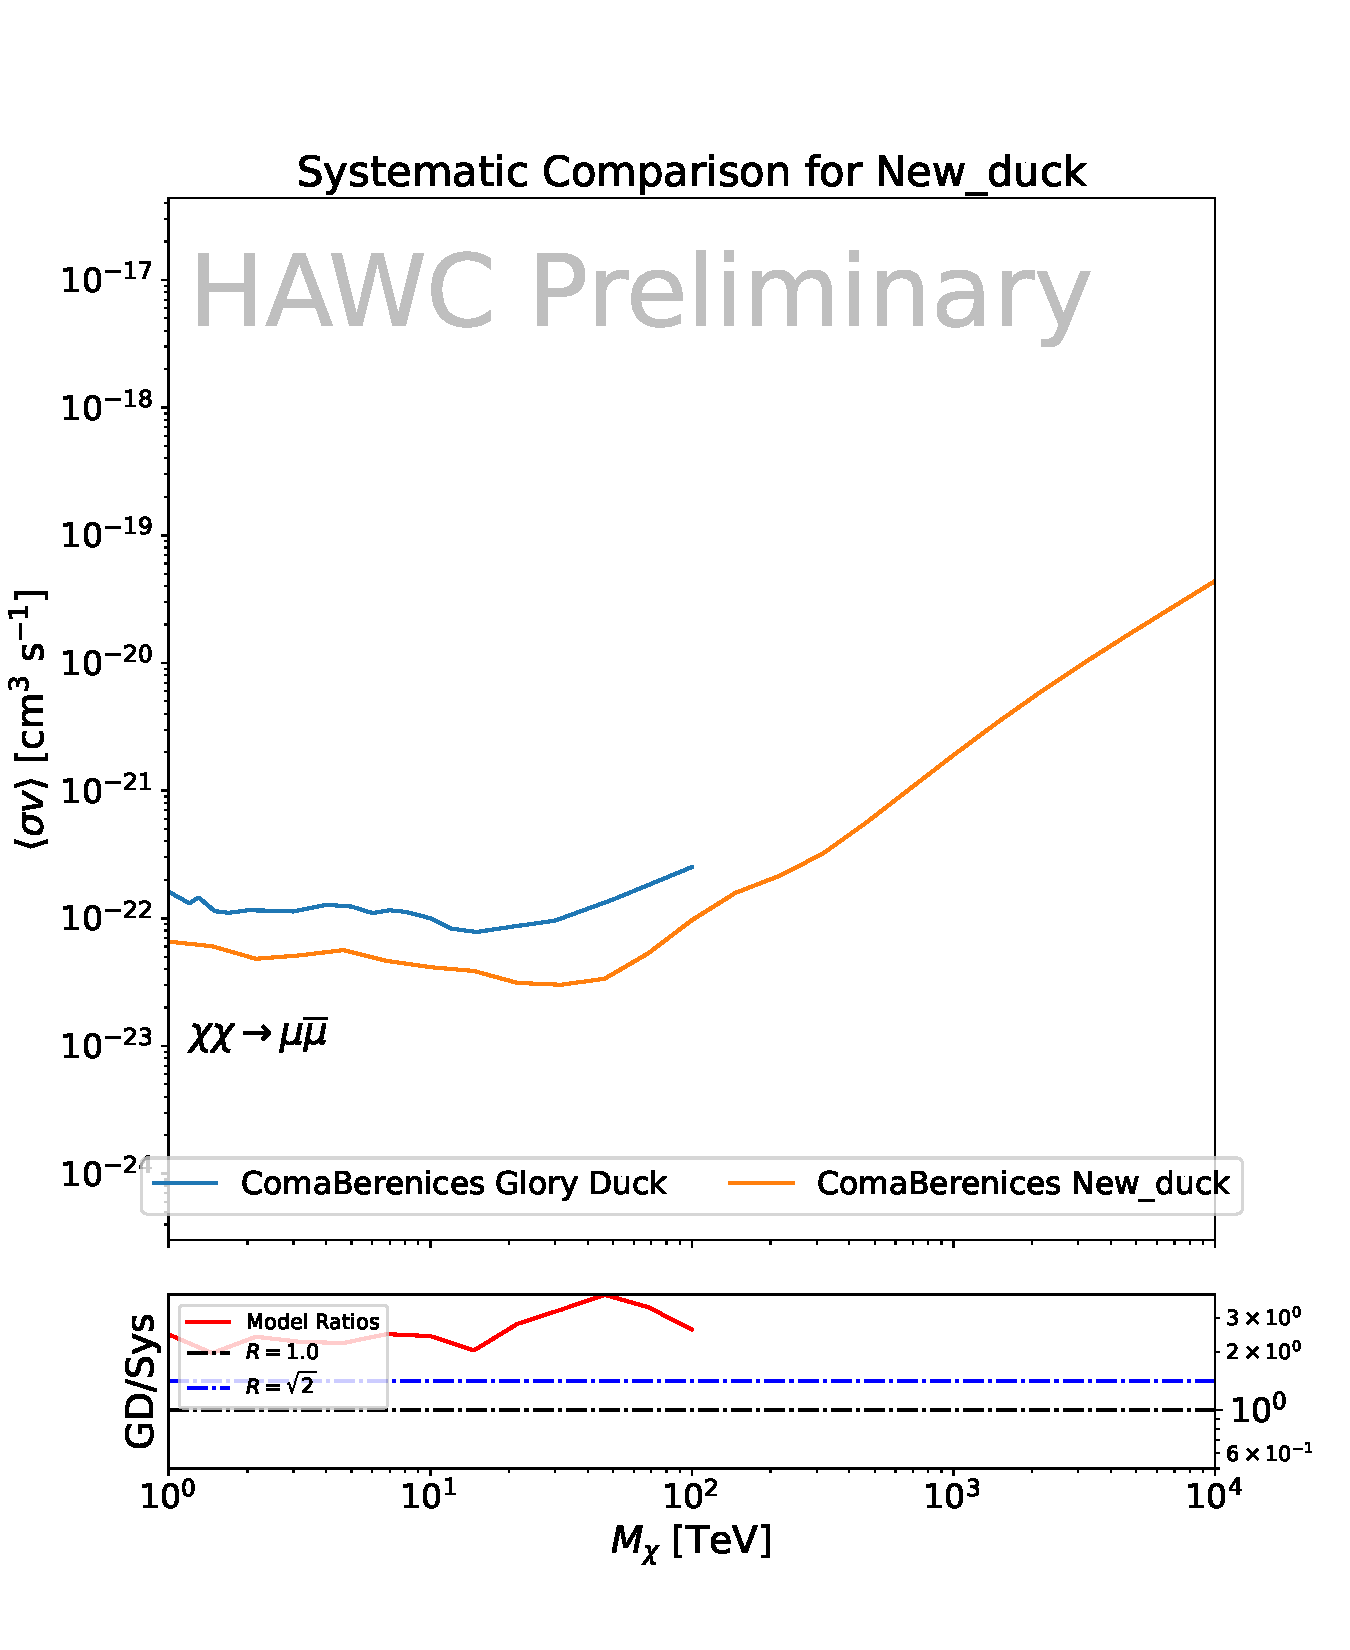
\includegraphics[scale=0.2]{figures/mtd_hawc_dm/systematics/Systematic_GD_New_duck_ComaBerenices_mumu.pdf}
    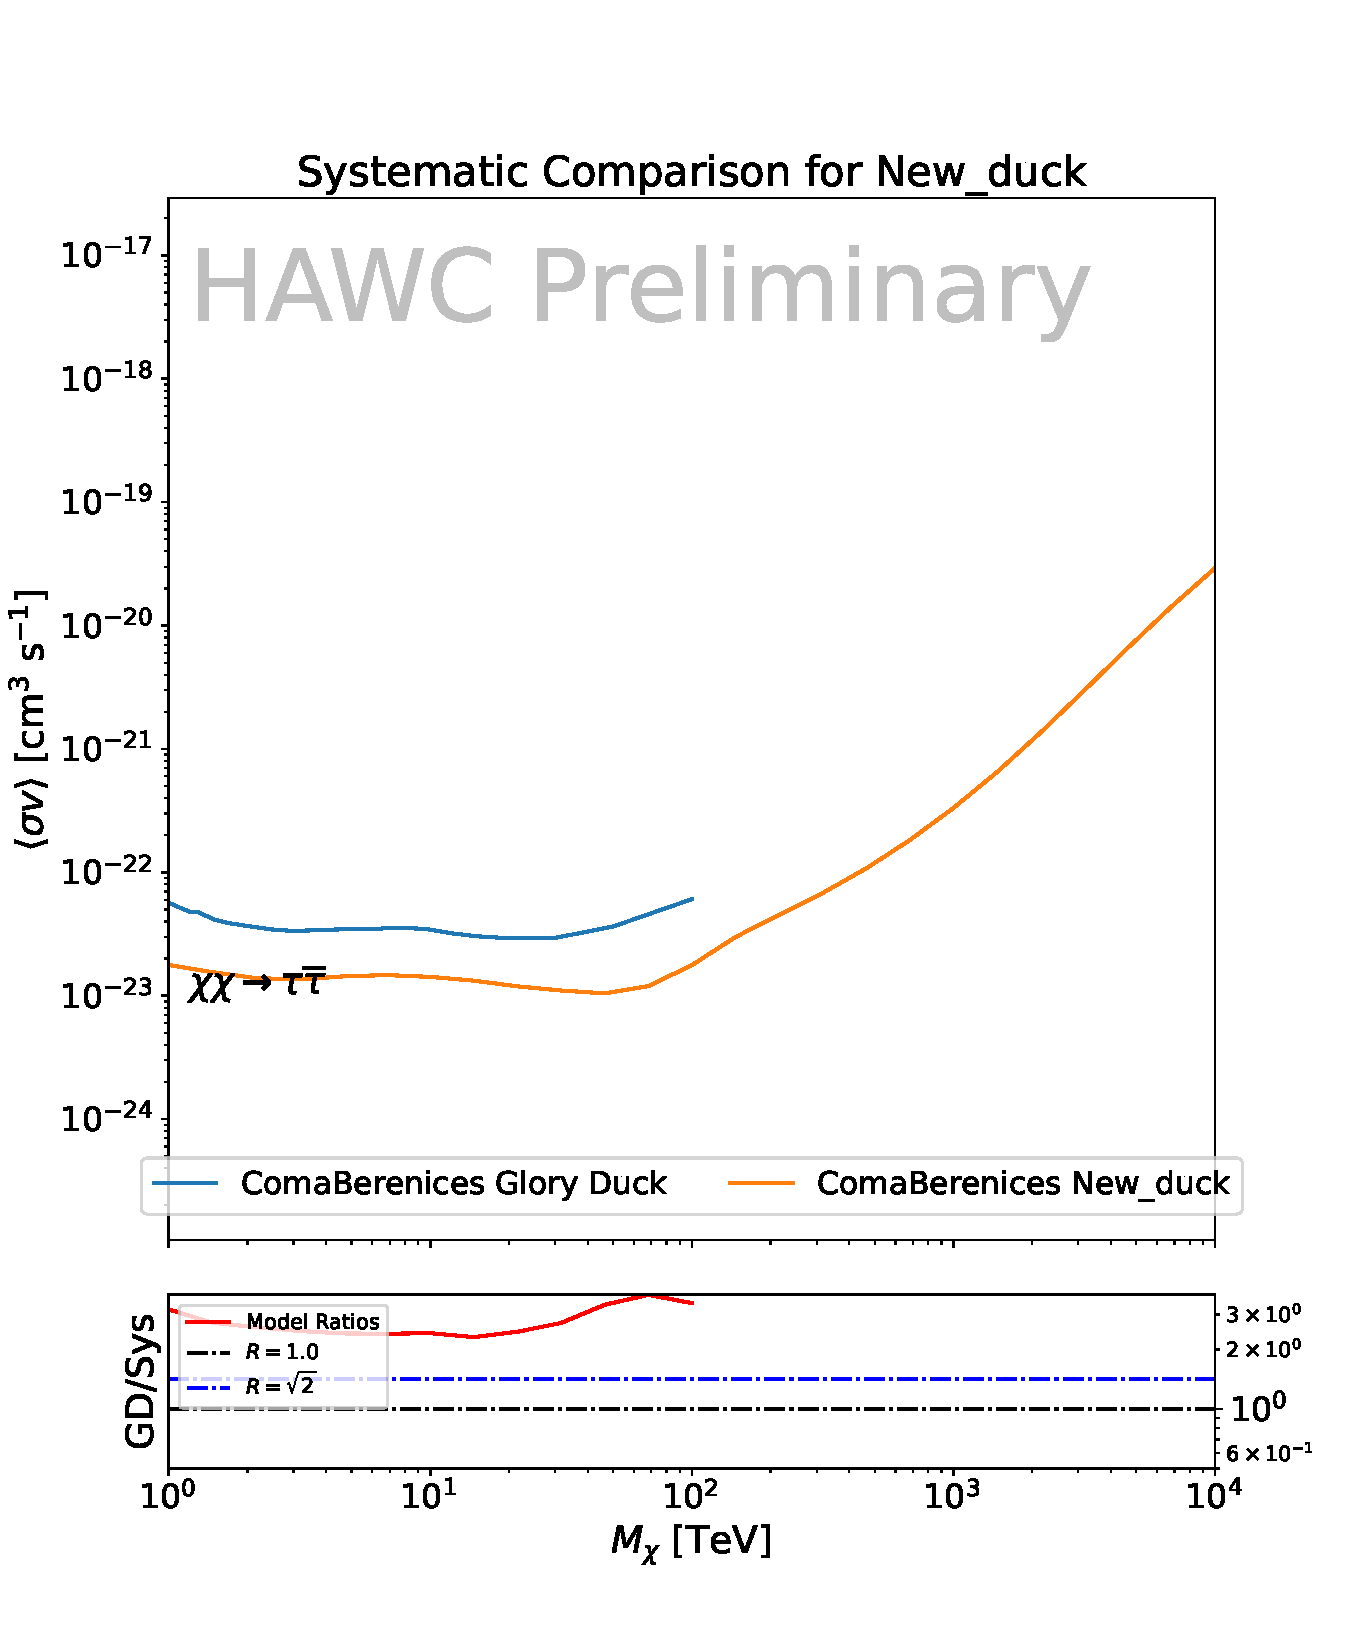
\includegraphics[scale=0.2]{figures/mtd_hawc_dm/systematics/Systematic_GD_New_duck_ComaBerenices_tautau.pdf}
    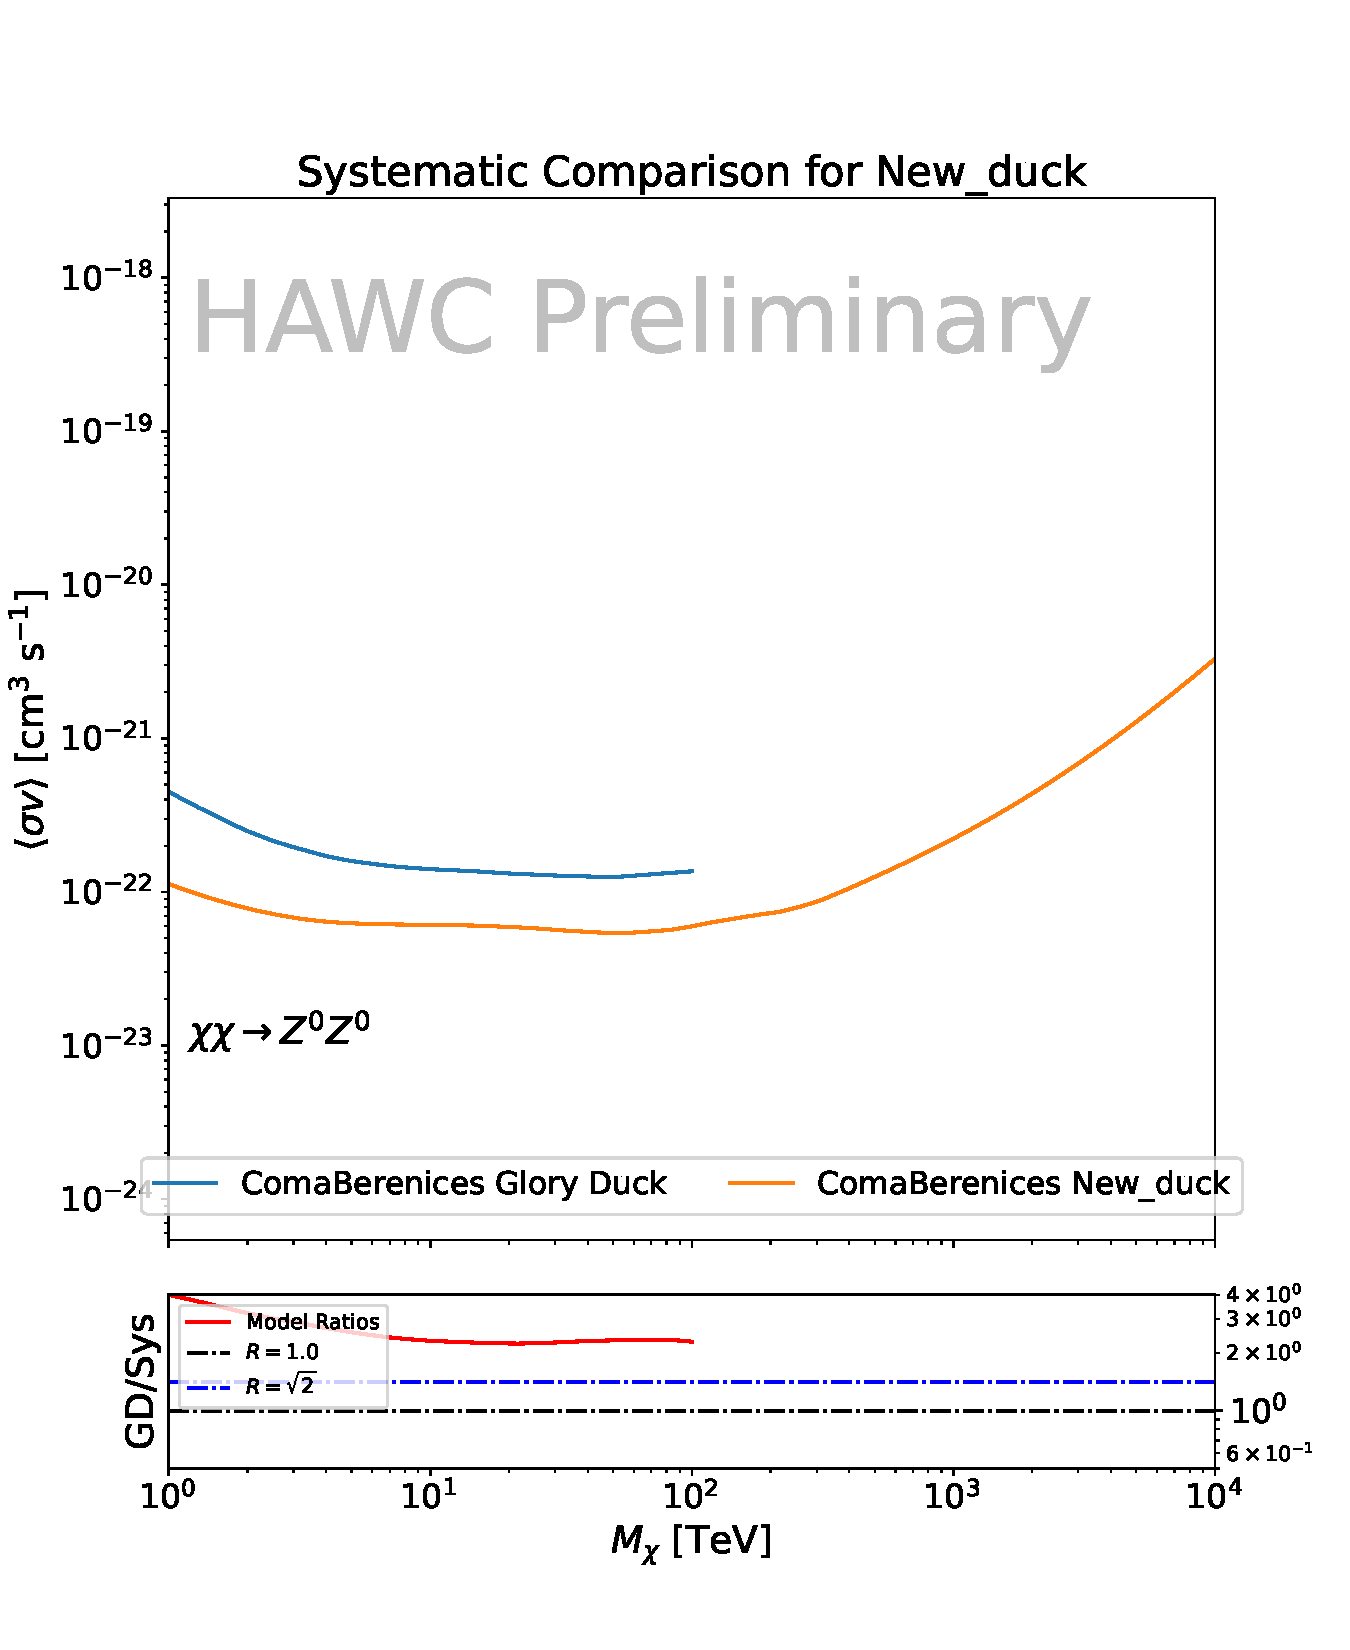
\includegraphics[scale=0.2]{figures/mtd_hawc_dm/systematics/Systematic_GD_New_duck_ComaBerenices_zz.pdf}
    }
    \caption{Comparison of HAWC limits from this analysis to Glory Duck (\cref{fig:hawc_combined_limit}) for Coma Berenices and 7 DM annihilation channels.}
\label{fig:mtd_compare_ComaB}
\end{figure}

\begin{figure}[h]
\centering{
    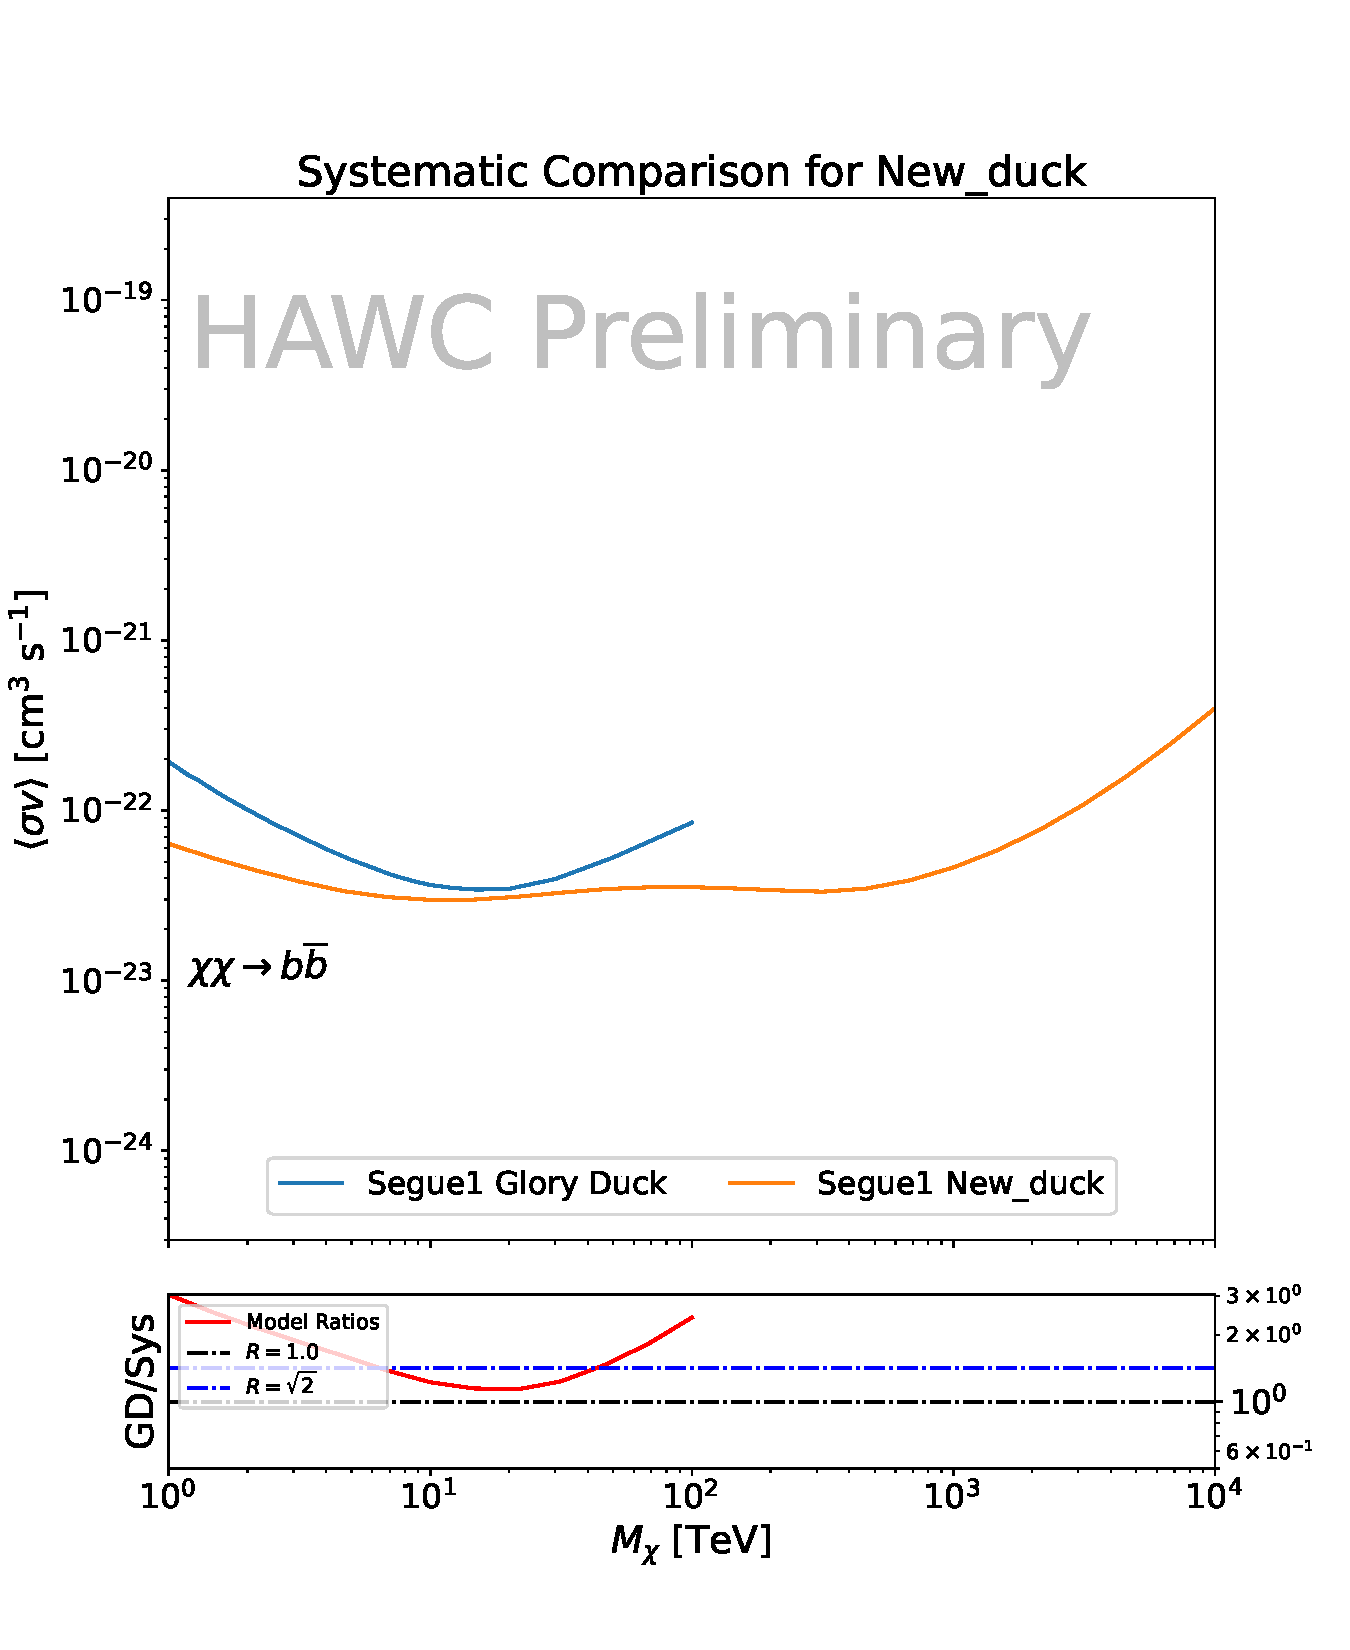
\includegraphics[scale=0.225]{figures/mtd_hawc_dm/systematics/Systematic_GD_New_duck_Segue1_bb.pdf}
    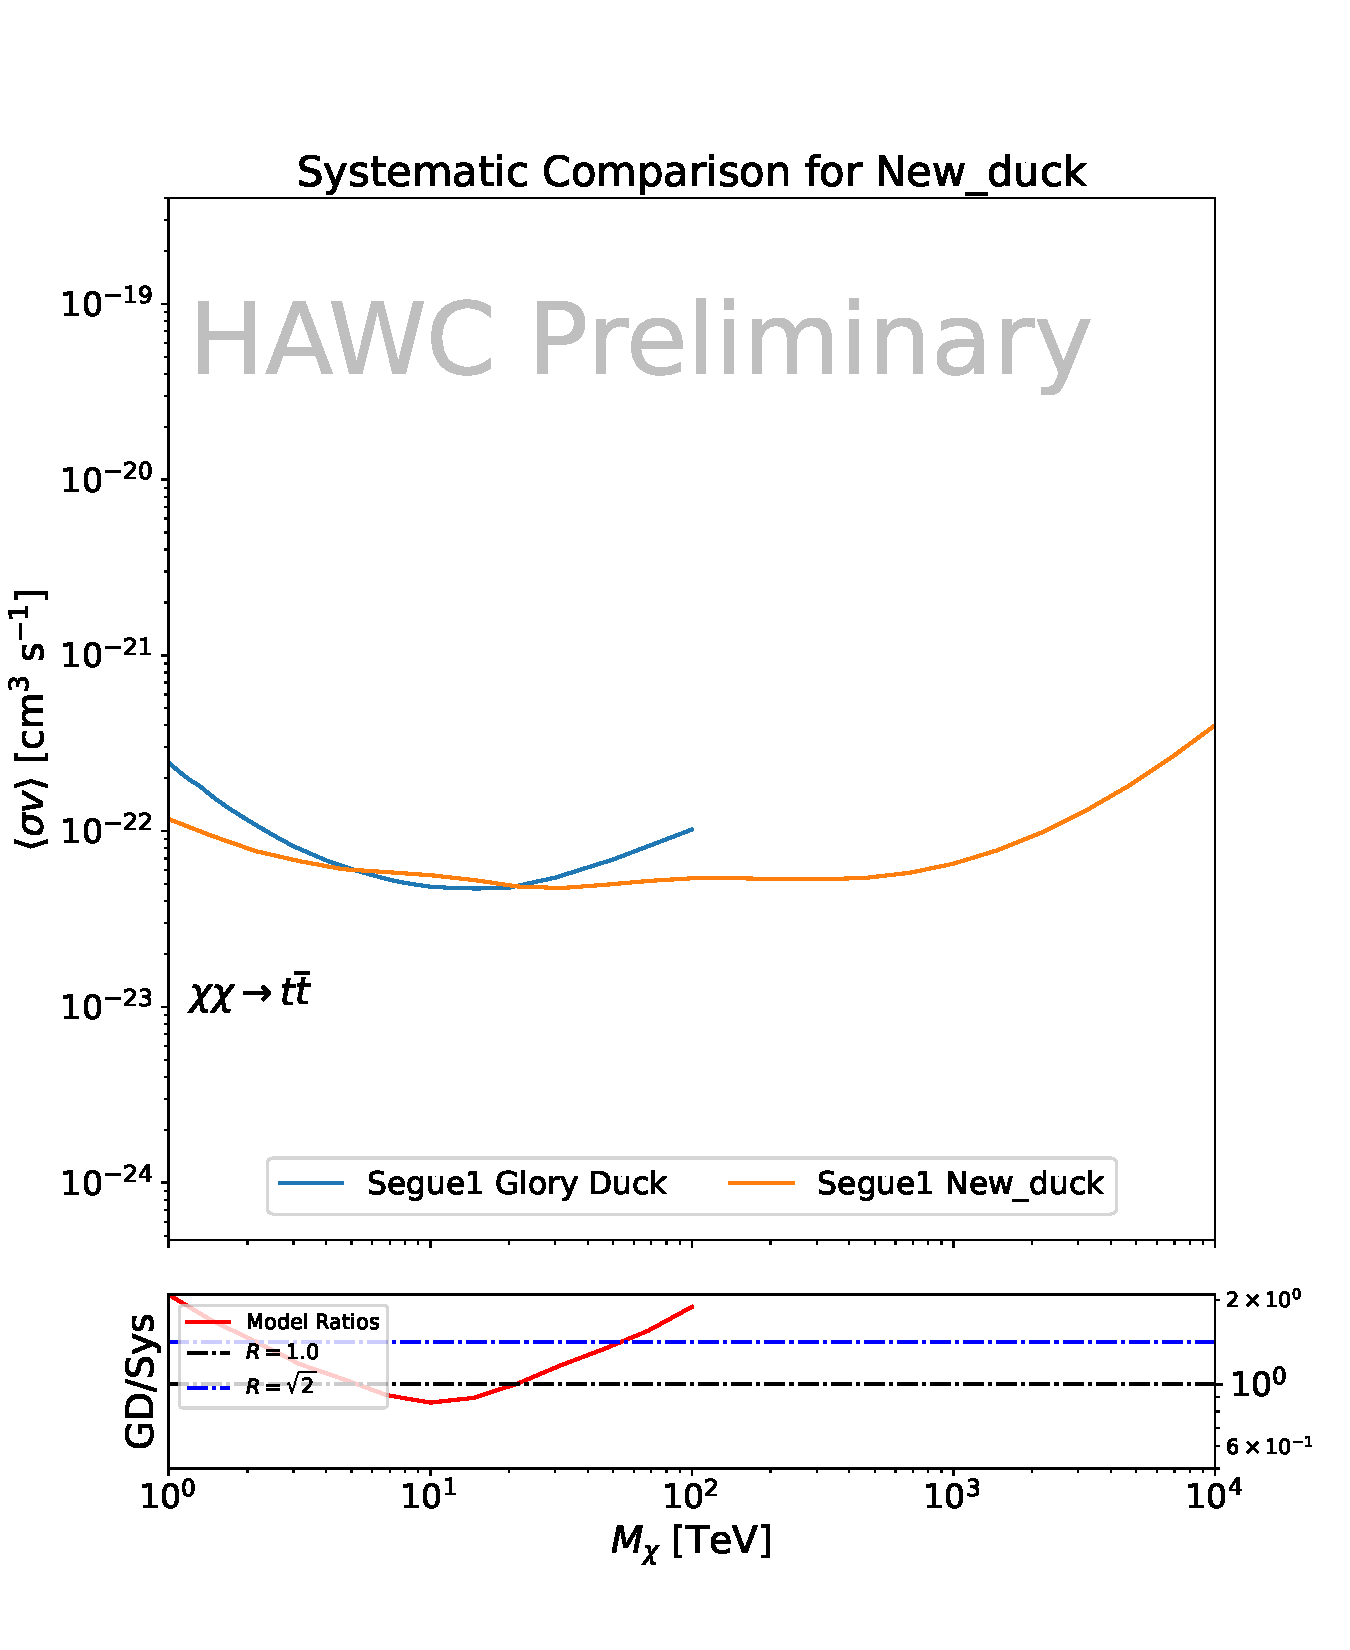
\includegraphics[scale=0.225]{figures/mtd_hawc_dm/systematics/Systematic_GD_New_duck_Segue1_tt.pdf}
    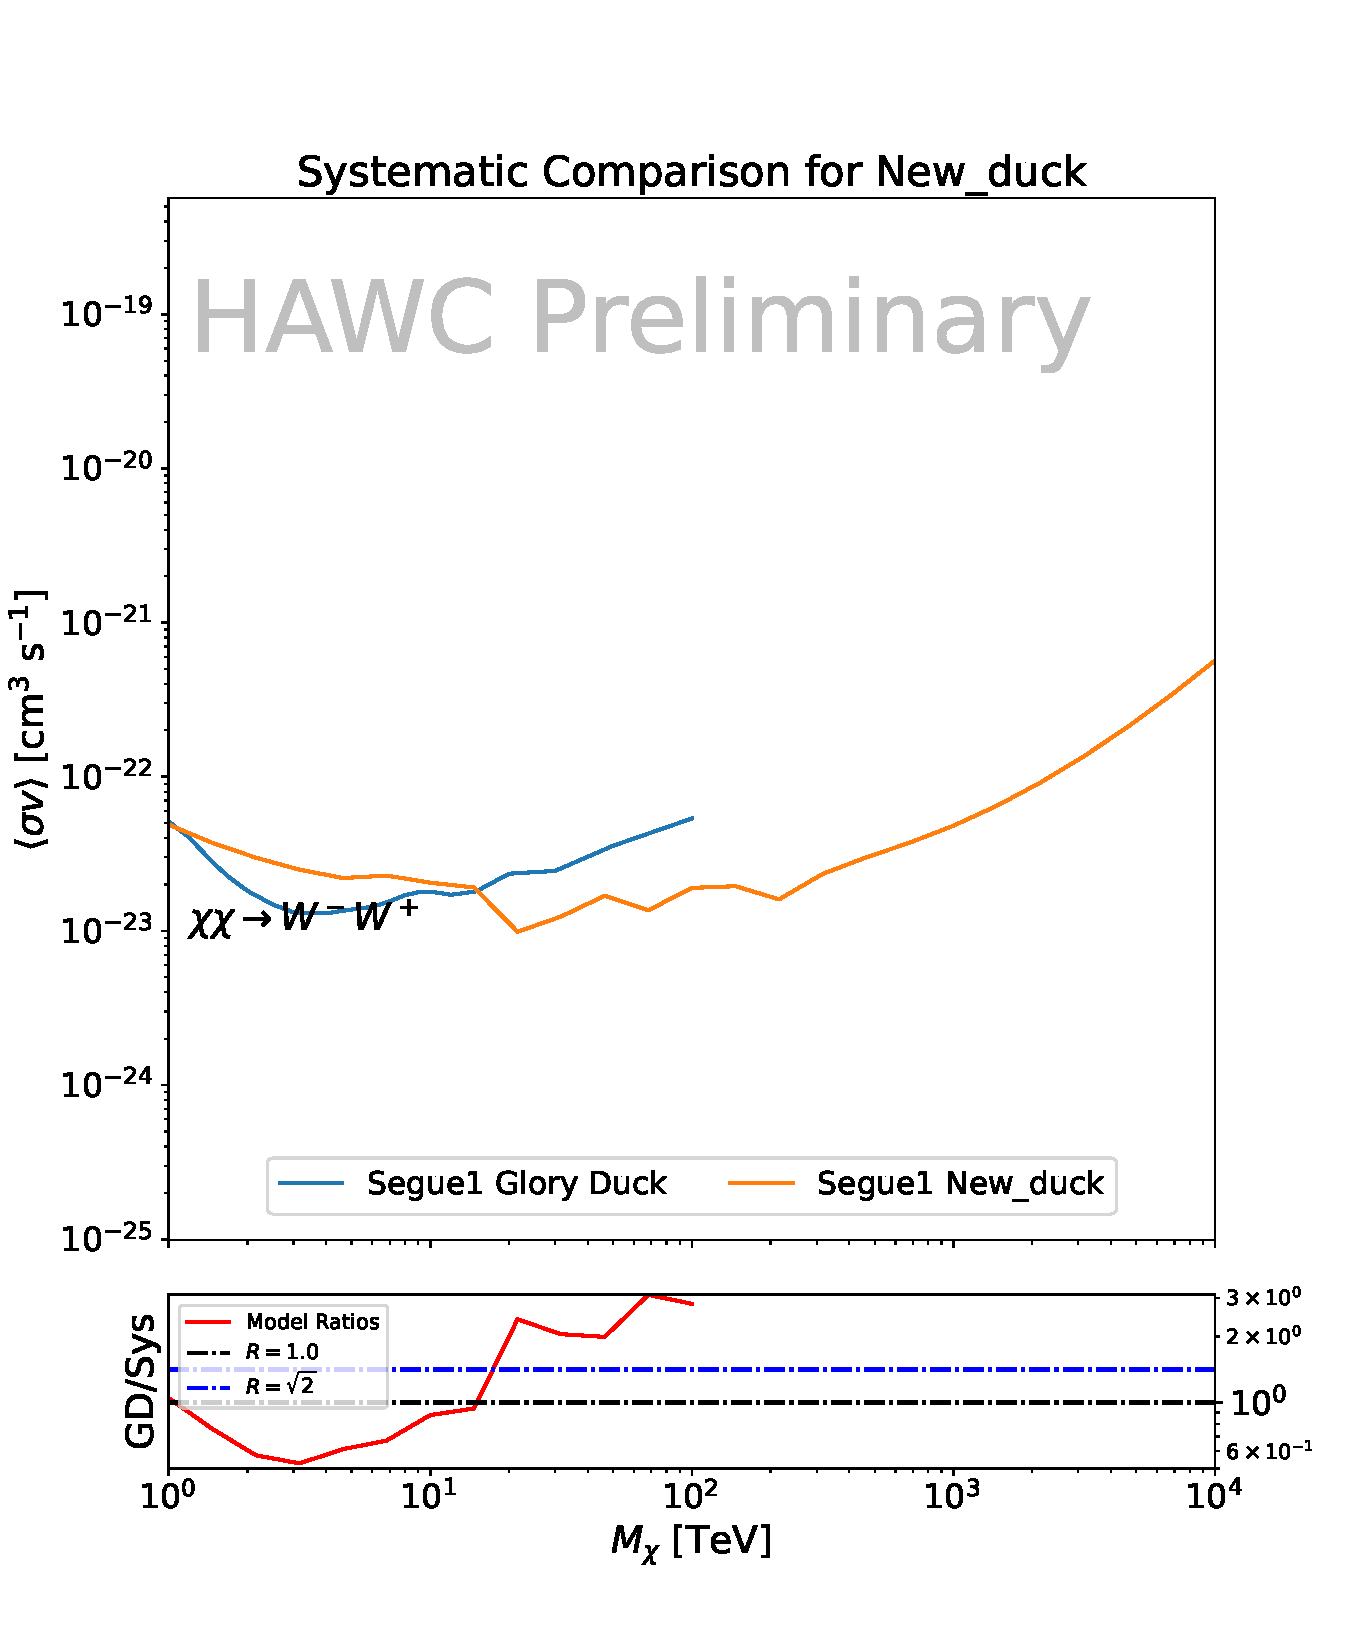
\includegraphics[scale=0.225]{figures/mtd_hawc_dm/systematics/Systematic_GD_New_duck_Segue1_ww.pdf}
    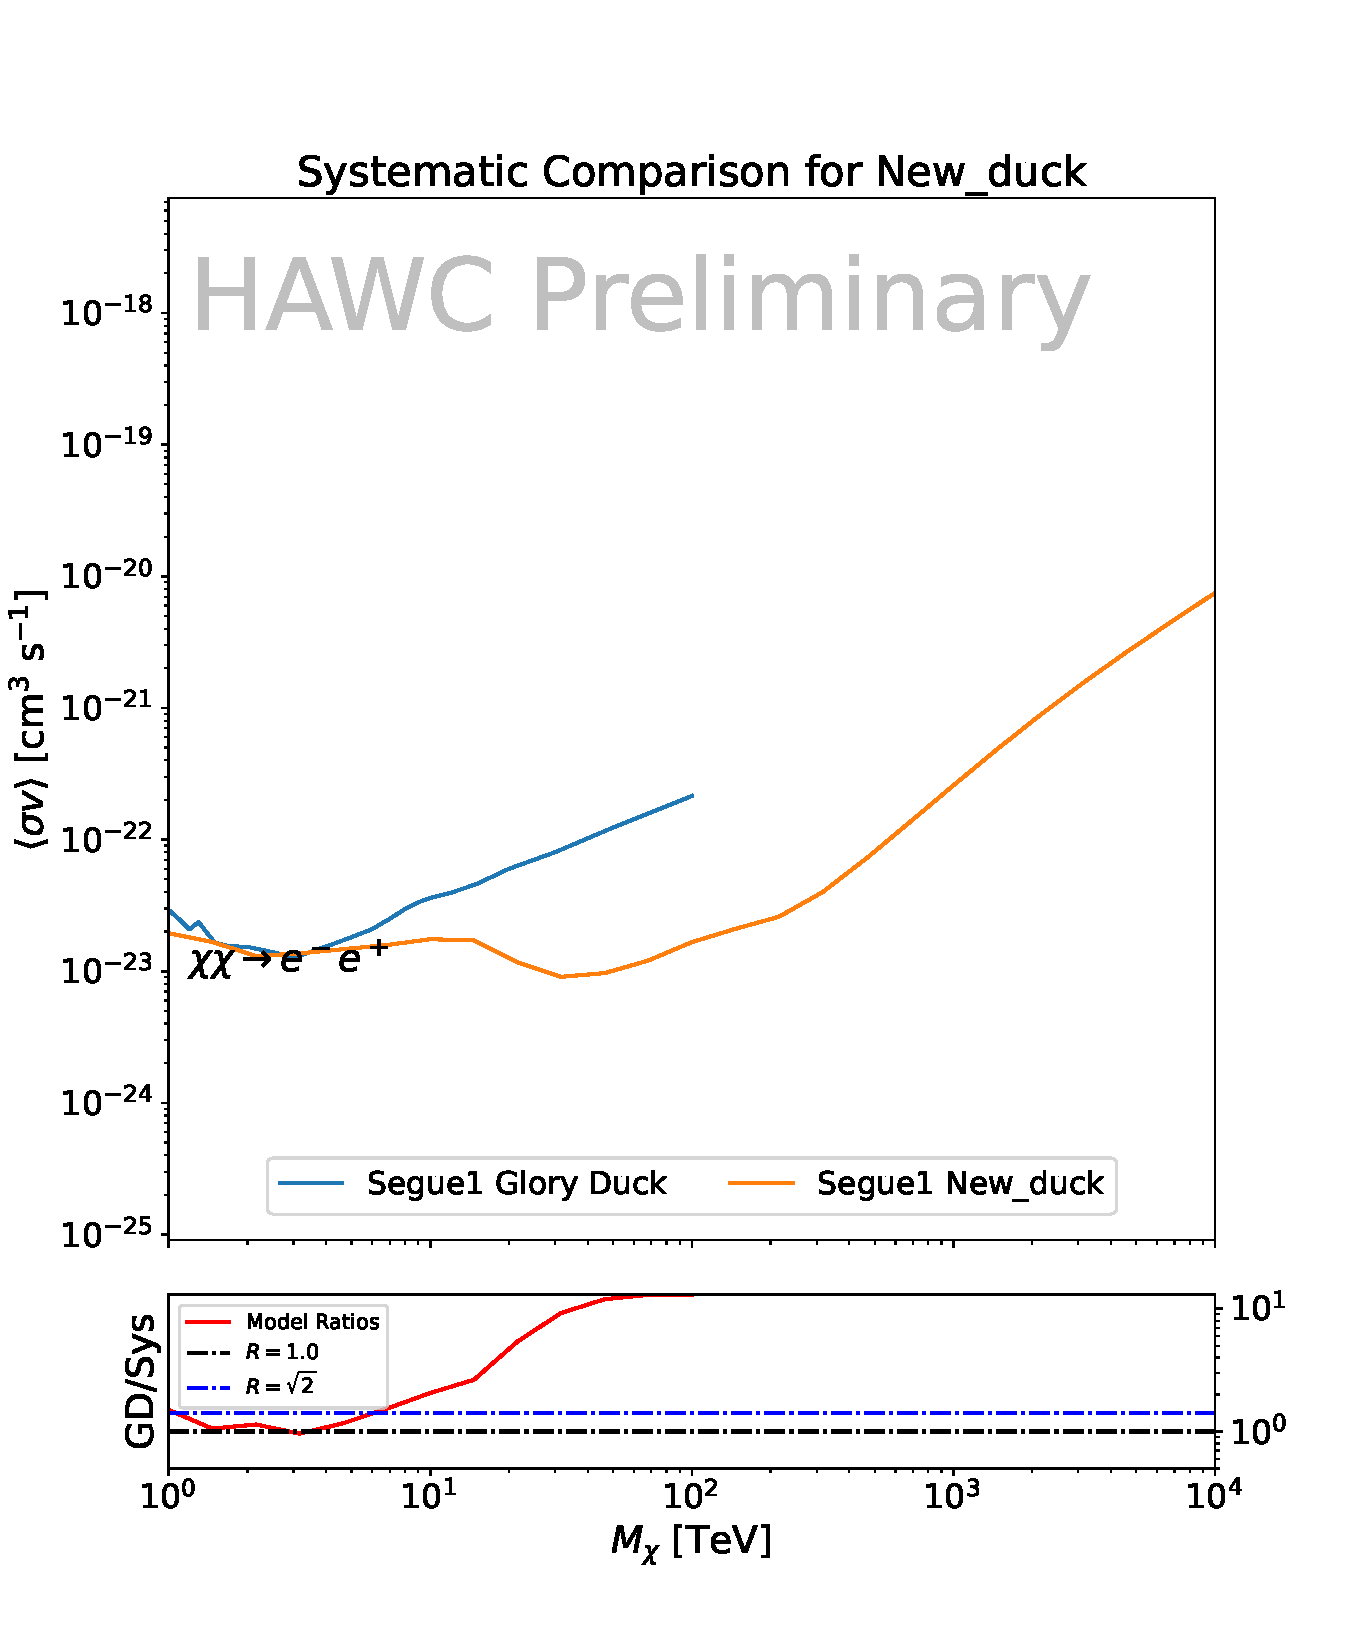
\includegraphics[scale=0.225]{figures/mtd_hawc_dm/systematics/Systematic_GD_New_duck_Segue1_ee.pdf}
    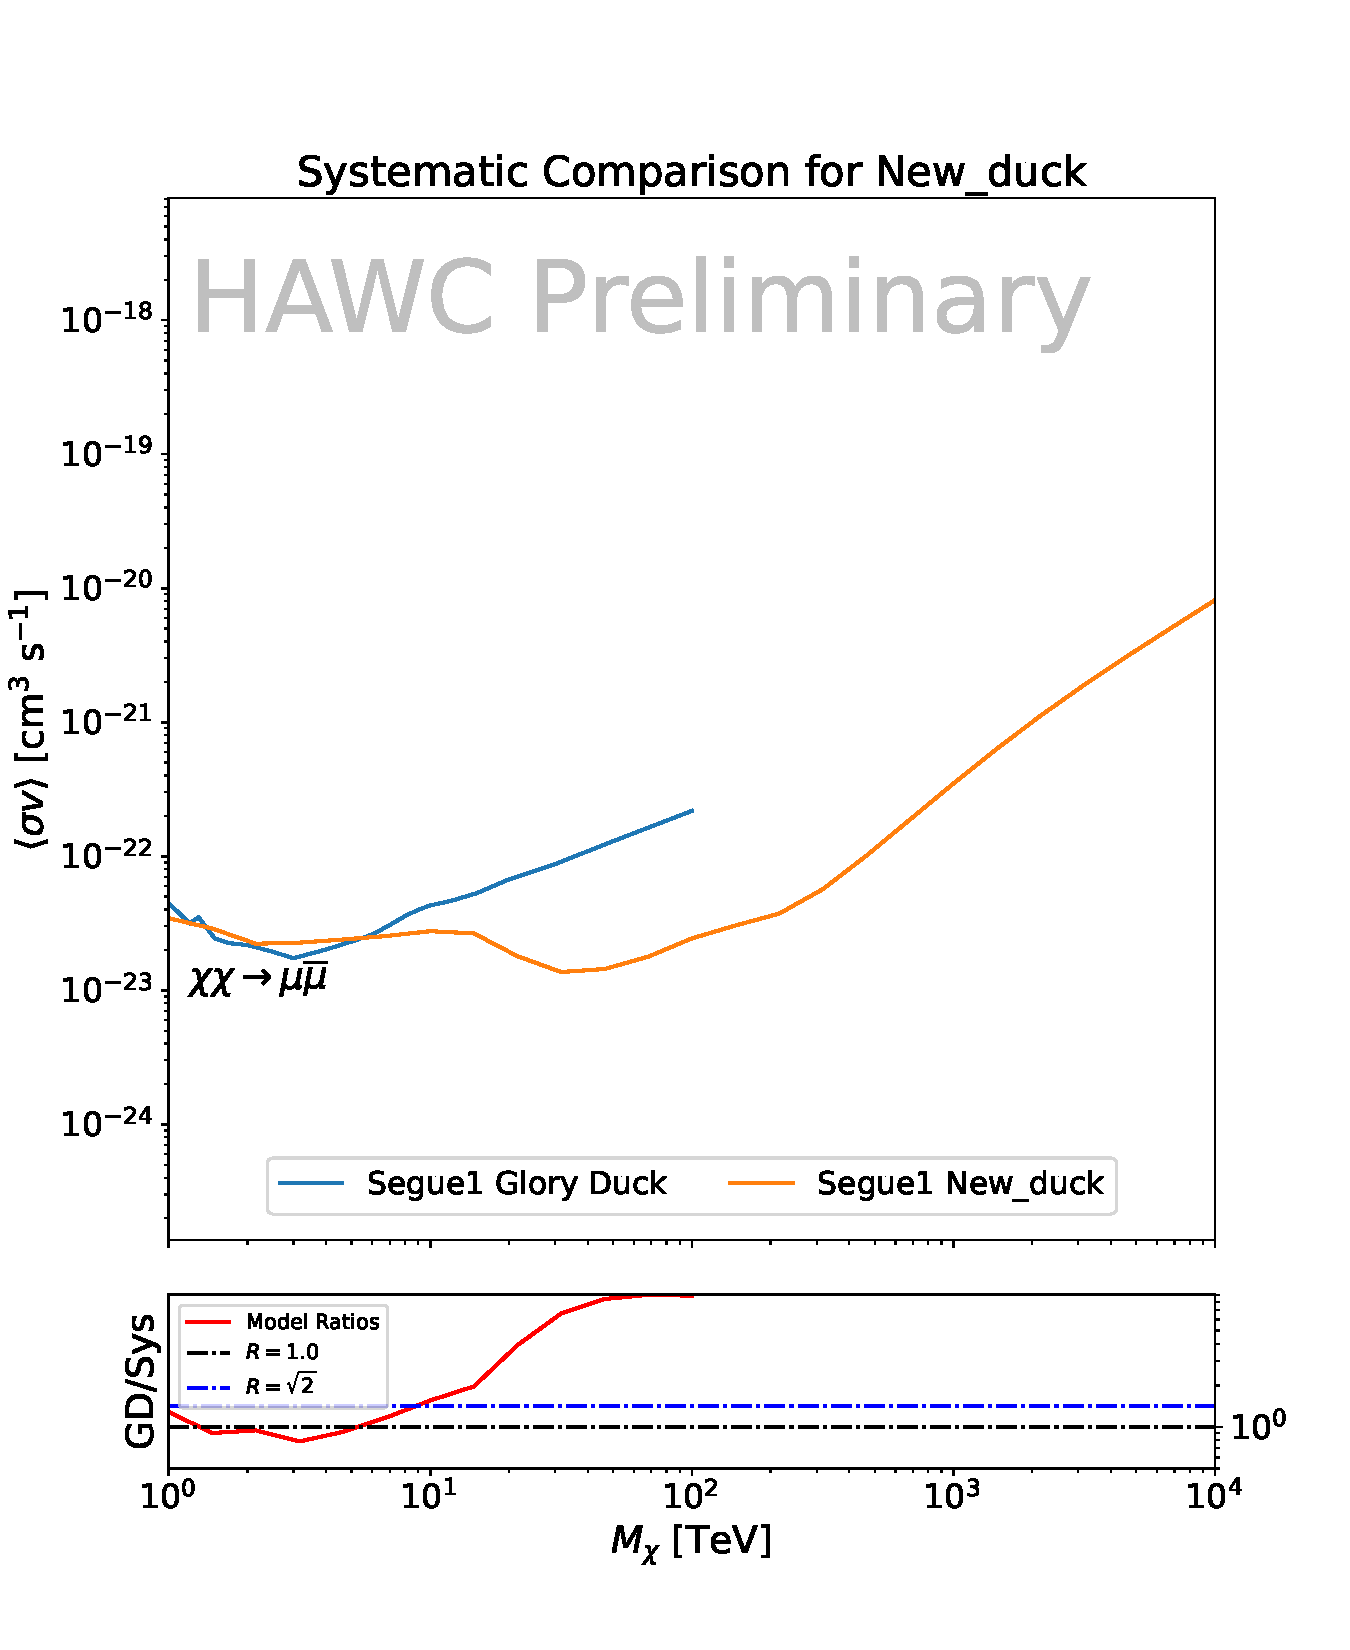
\includegraphics[scale=0.225]{figures/mtd_hawc_dm/systematics/Systematic_GD_New_duck_Segue1_mumu.pdf}
    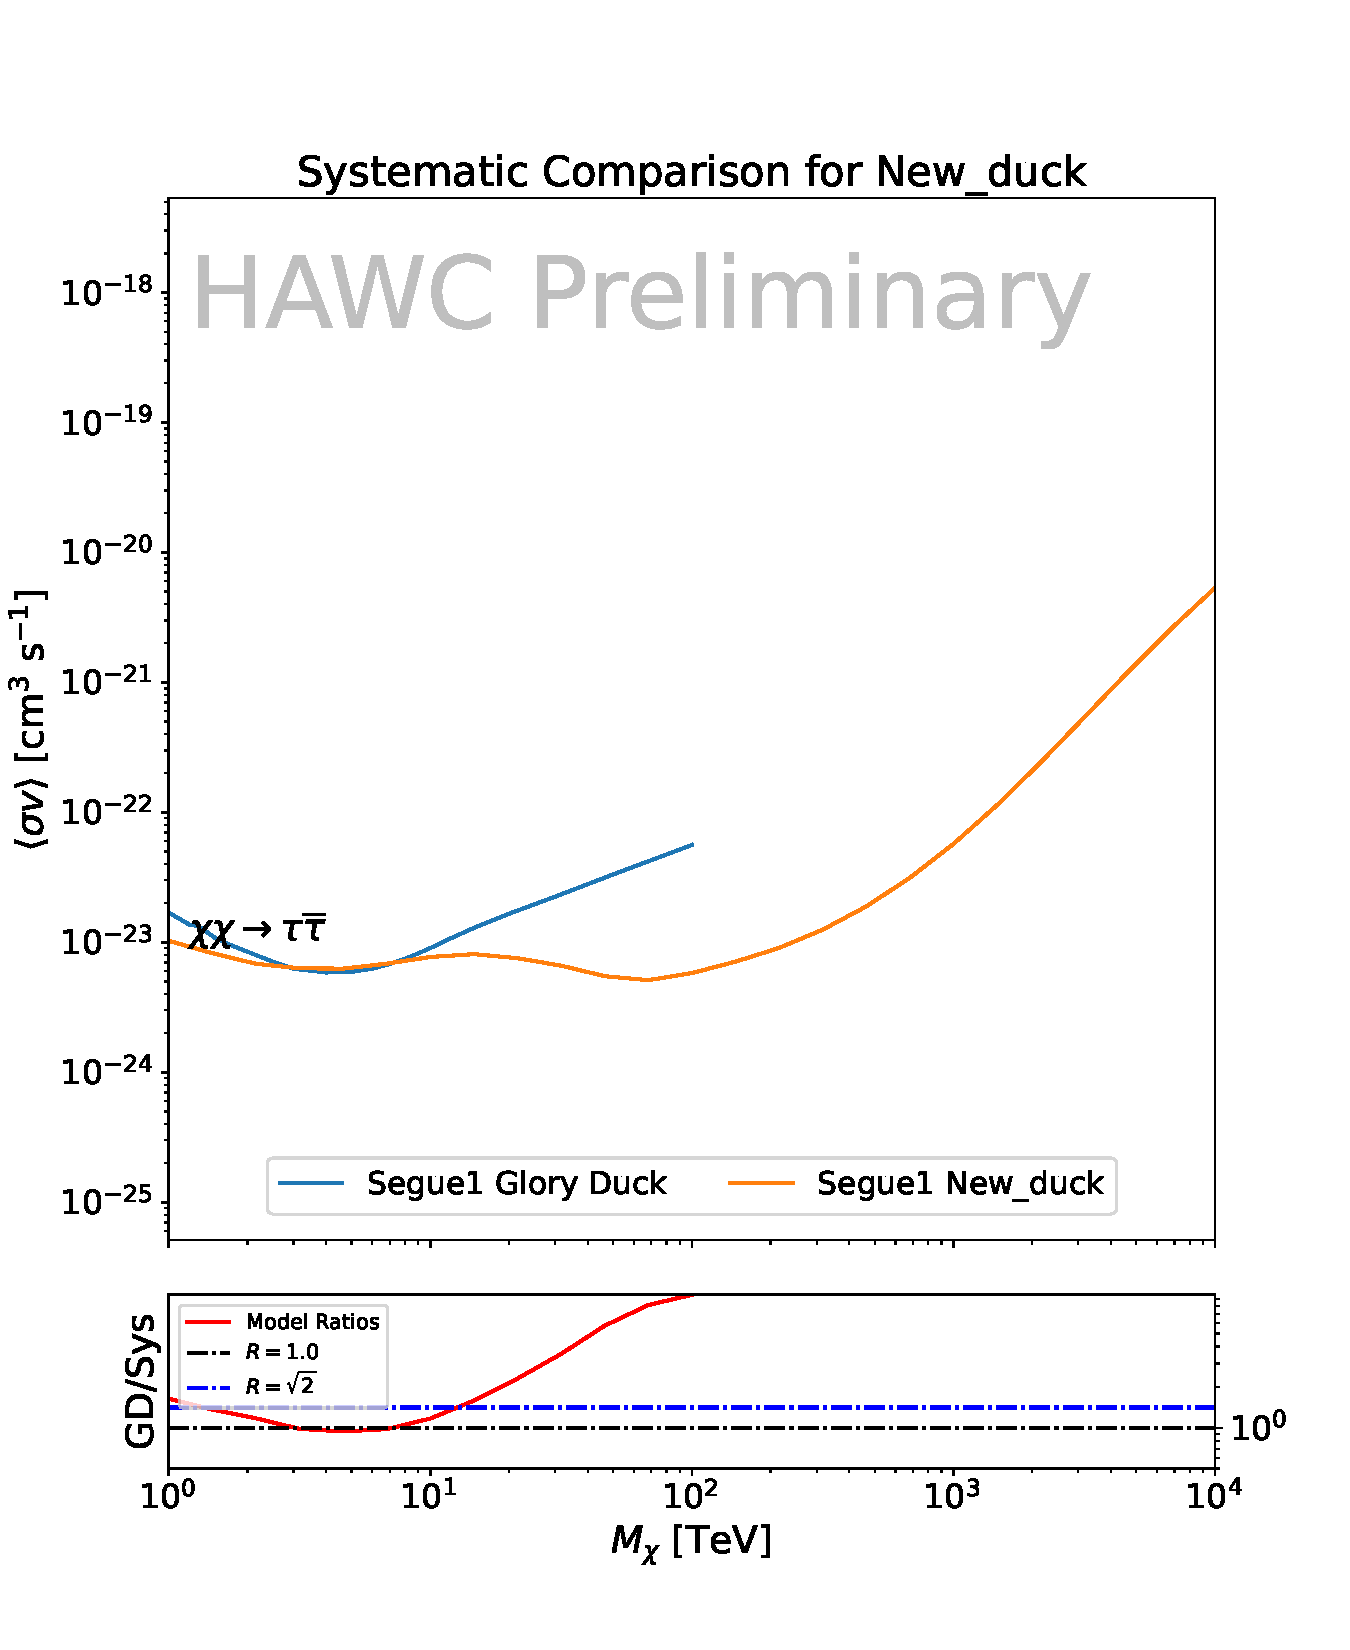
\includegraphics[scale=0.225]{figures/mtd_hawc_dm/systematics/Systematic_GD_New_duck_Segue1_tautau.pdf}
    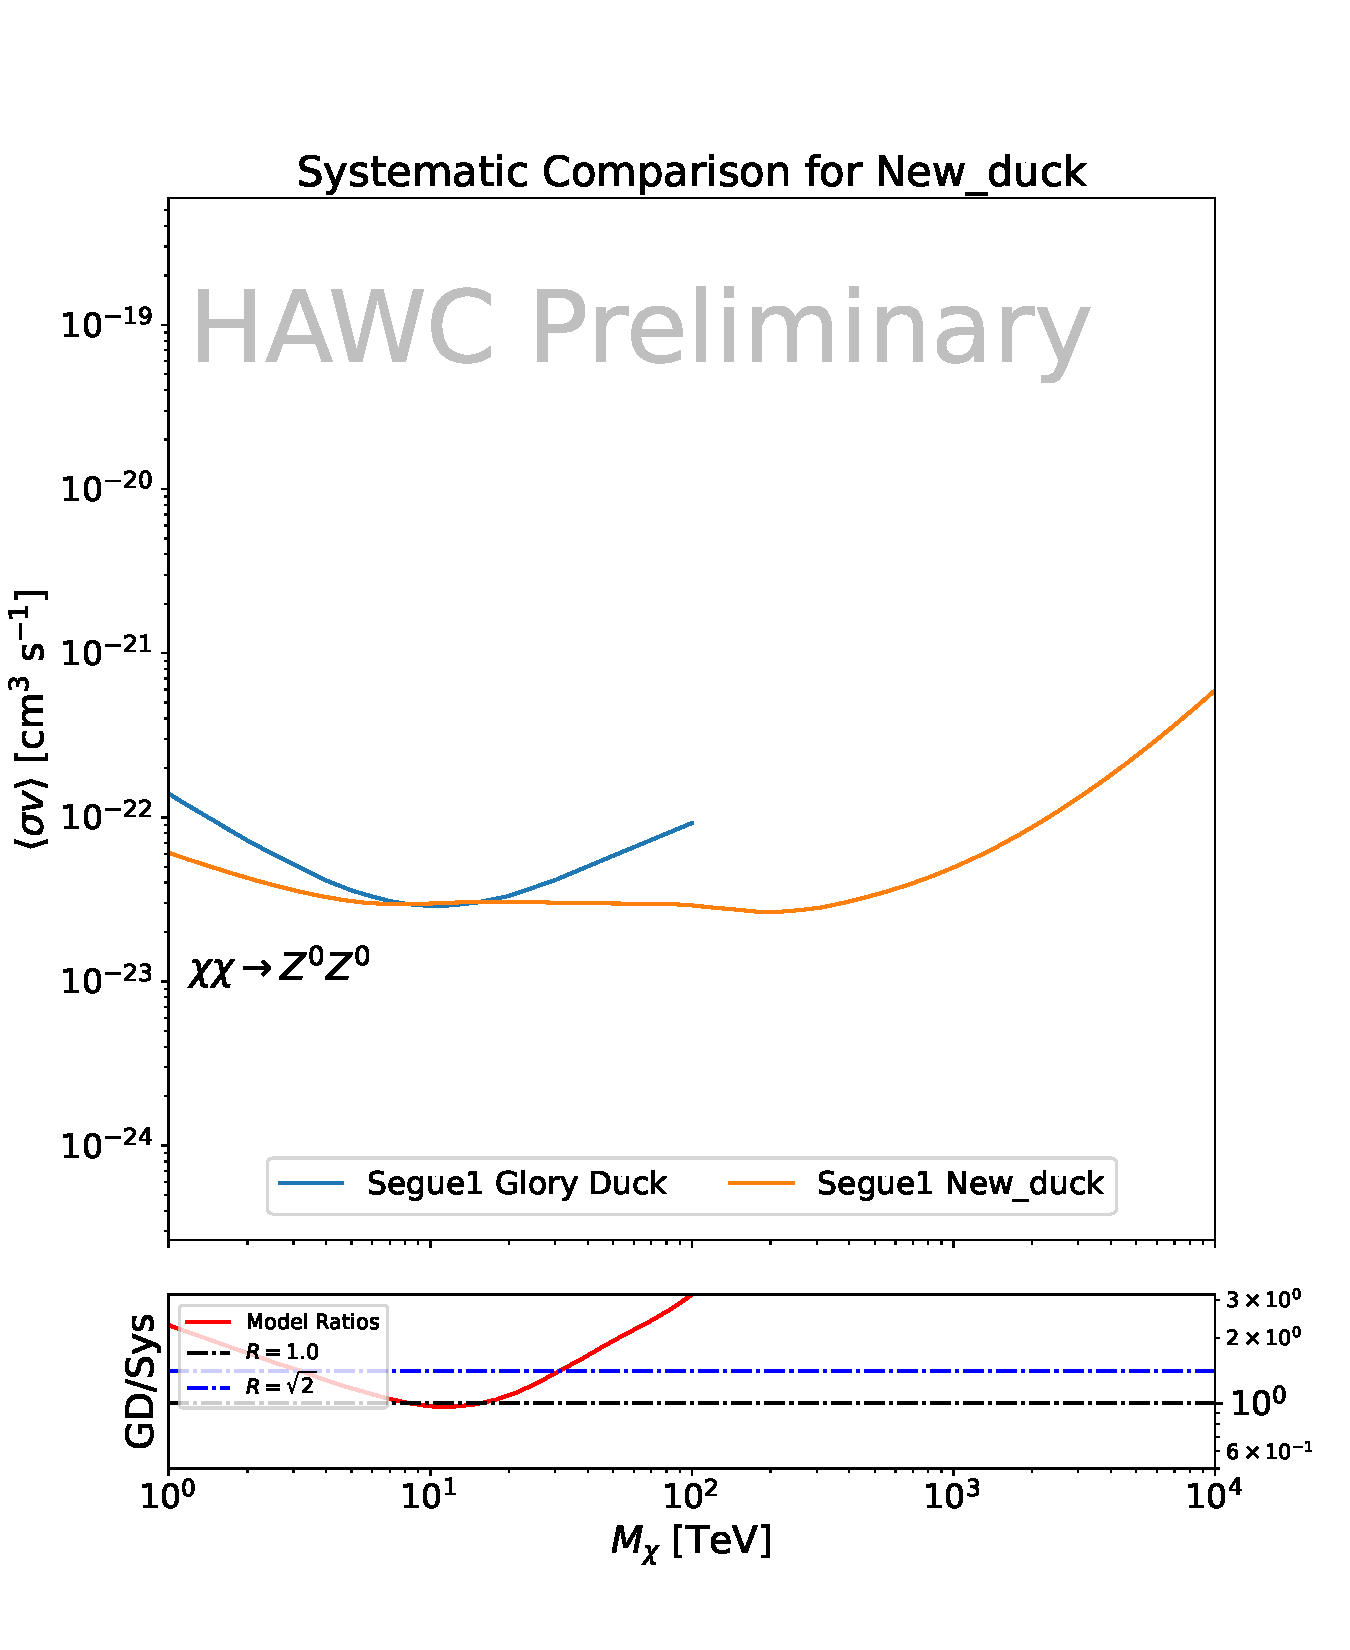
\includegraphics[scale=0.225]{figures/mtd_hawc_dm/systematics/Systematic_GD_New_duck_Segue1_zz.pdf}
    }
    \caption{Same as \cref{fig:mtd_compare_ComaB} but for Segue 1.}
\label{fig:mtd_compare_Seg1}
\end{figure}

\begin{figure}[h]
\centering{
    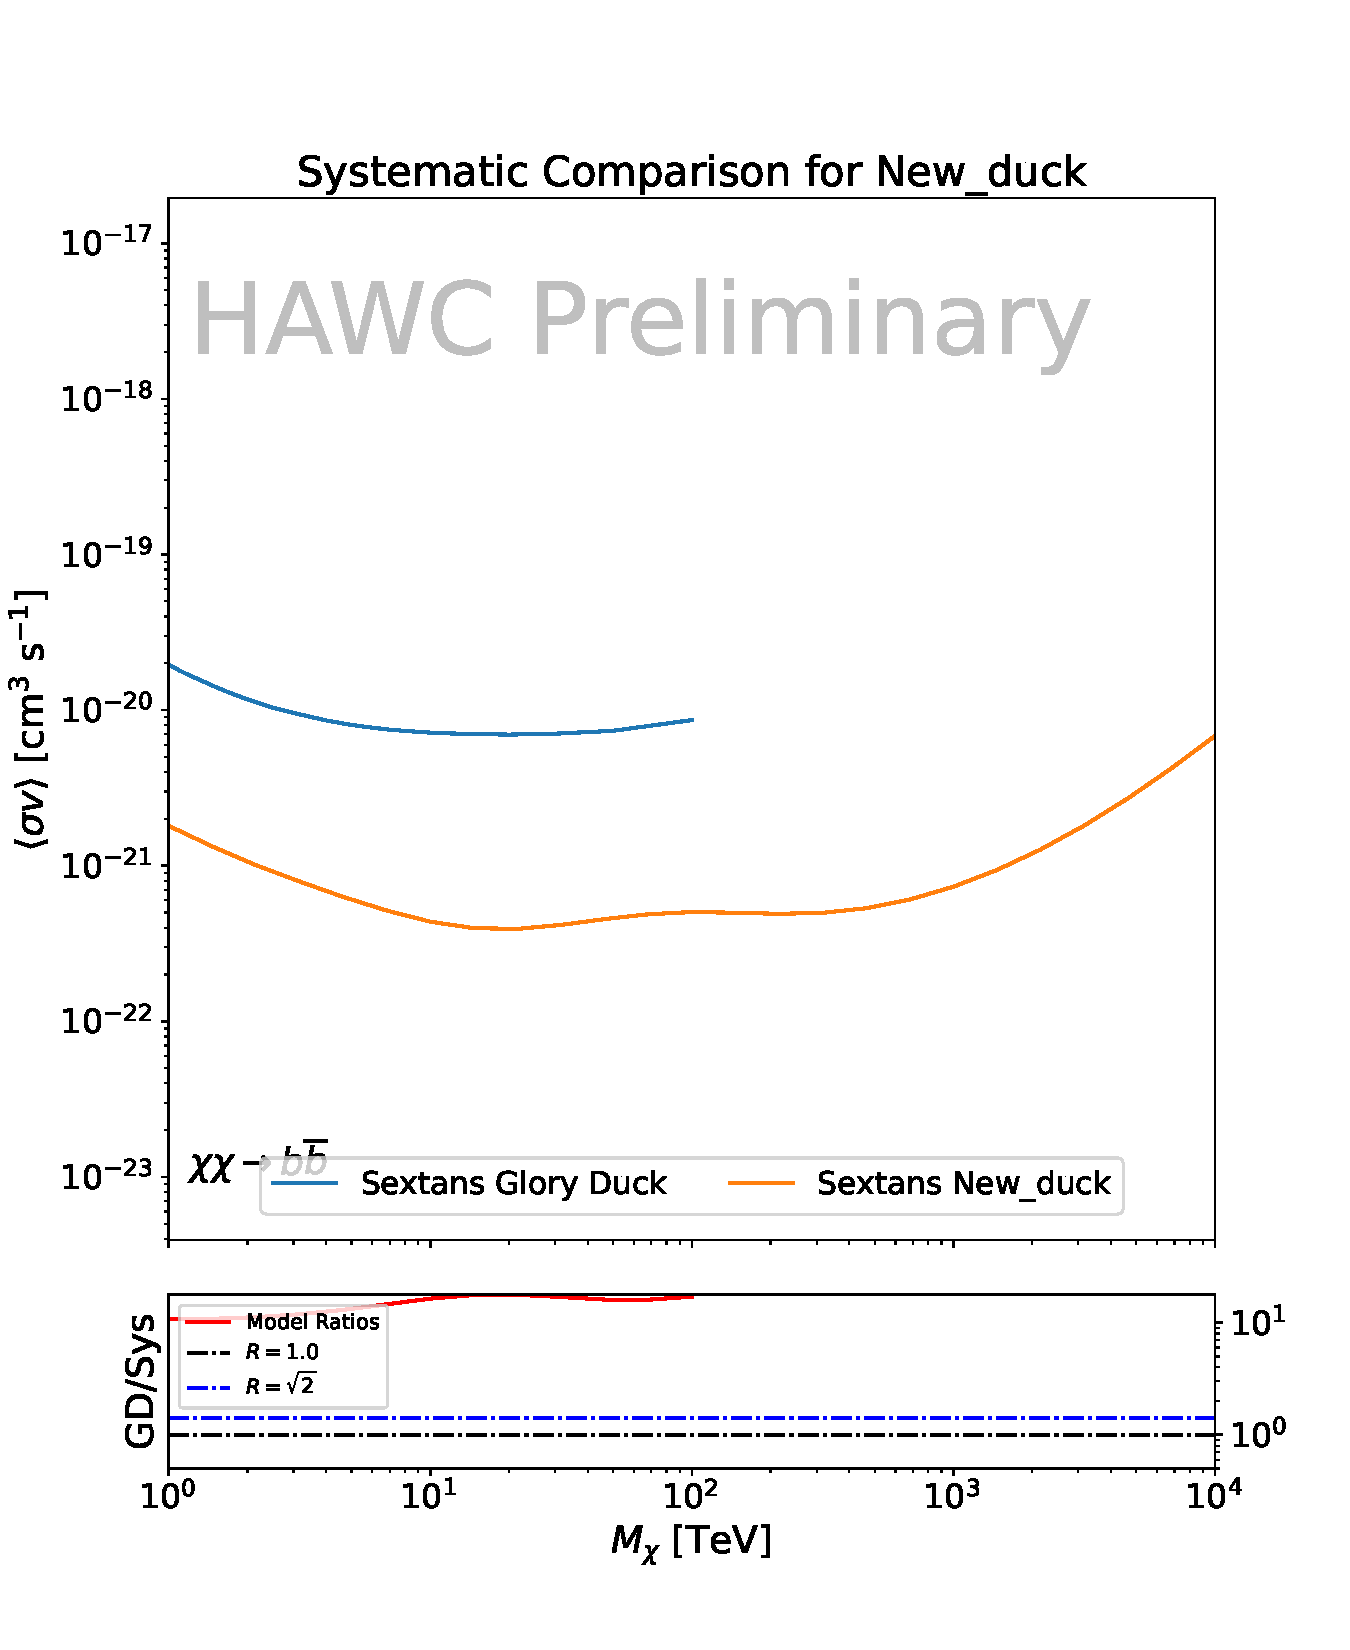
\includegraphics[scale=0.225]{figures/mtd_hawc_dm/systematics/Systematic_GD_New_duck_Sextans_bb.pdf}
    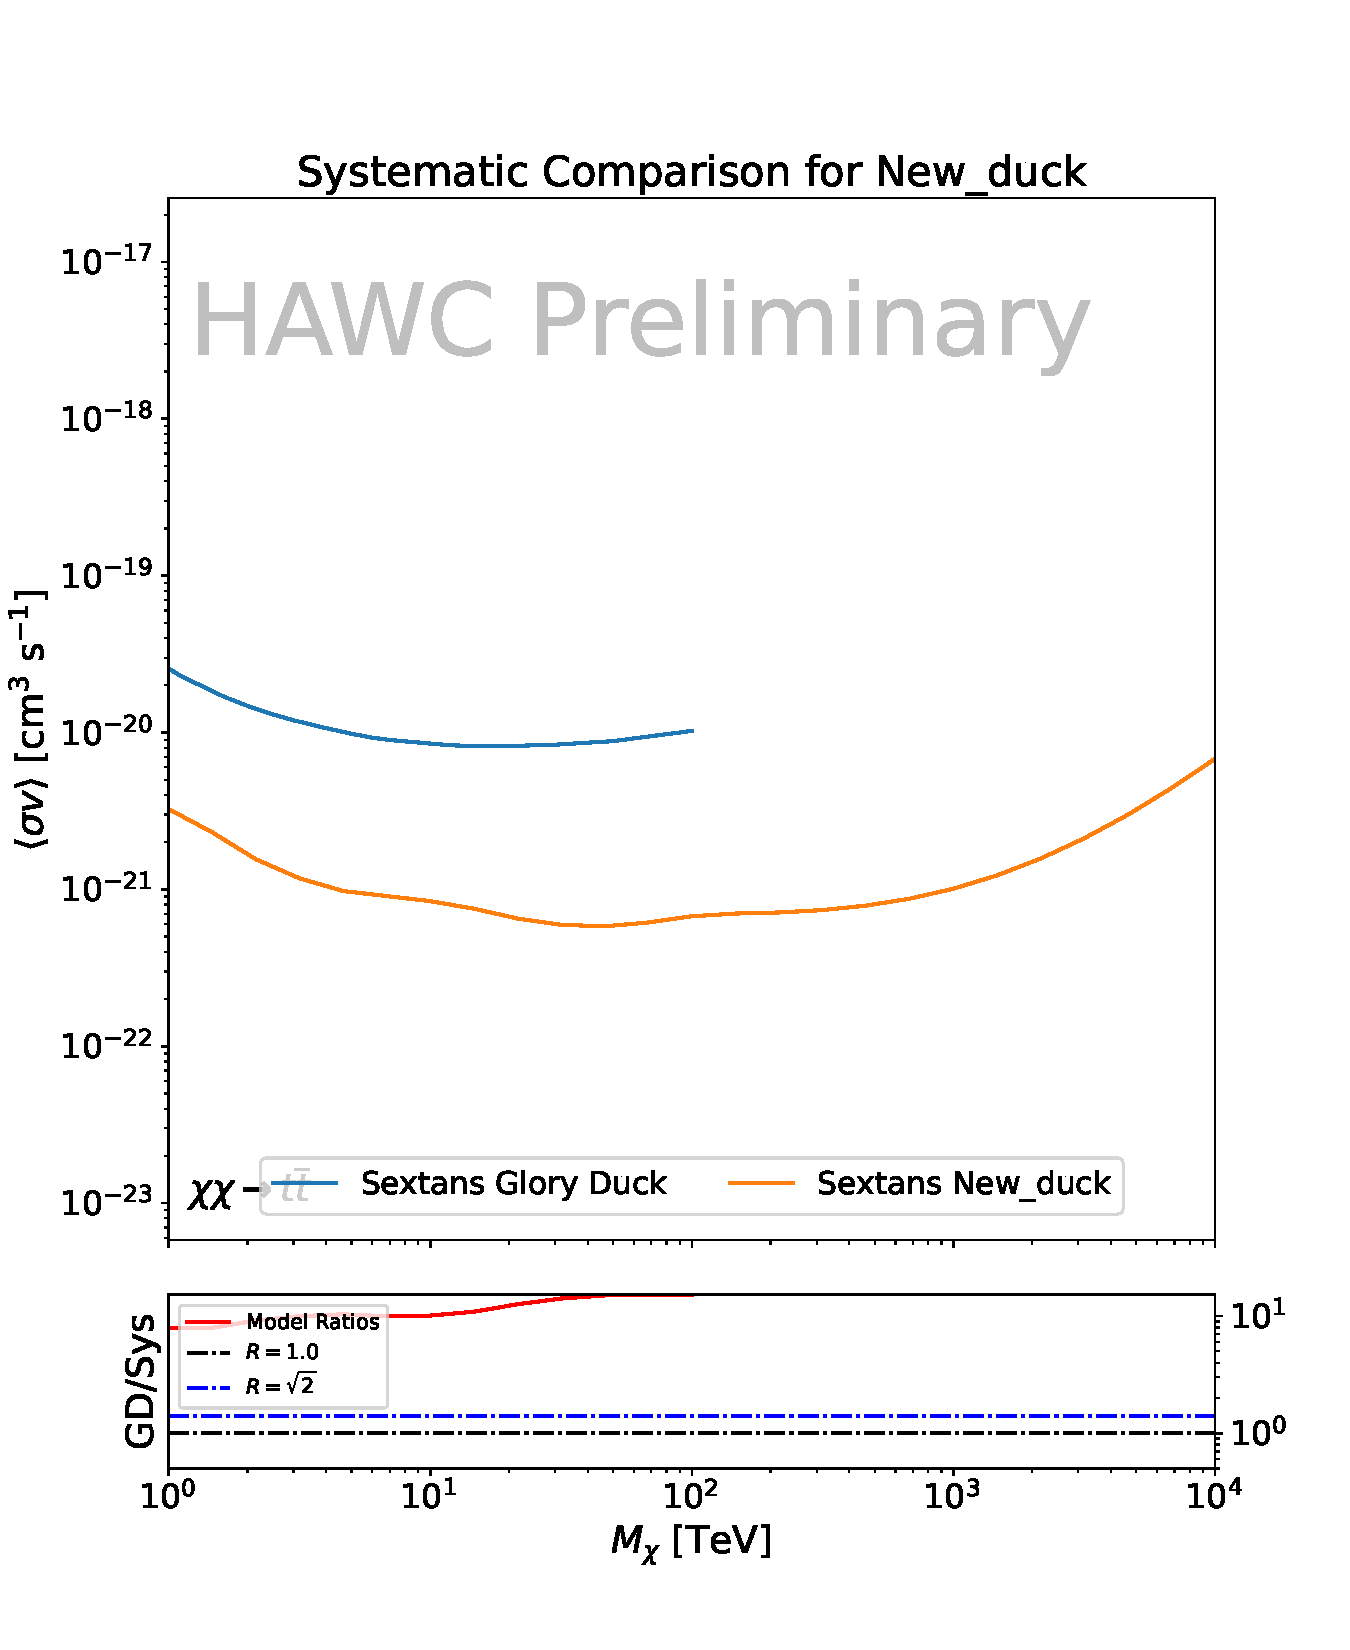
\includegraphics[scale=0.225]{figures/mtd_hawc_dm/systematics/Systematic_GD_New_duck_Sextans_tt.pdf}
    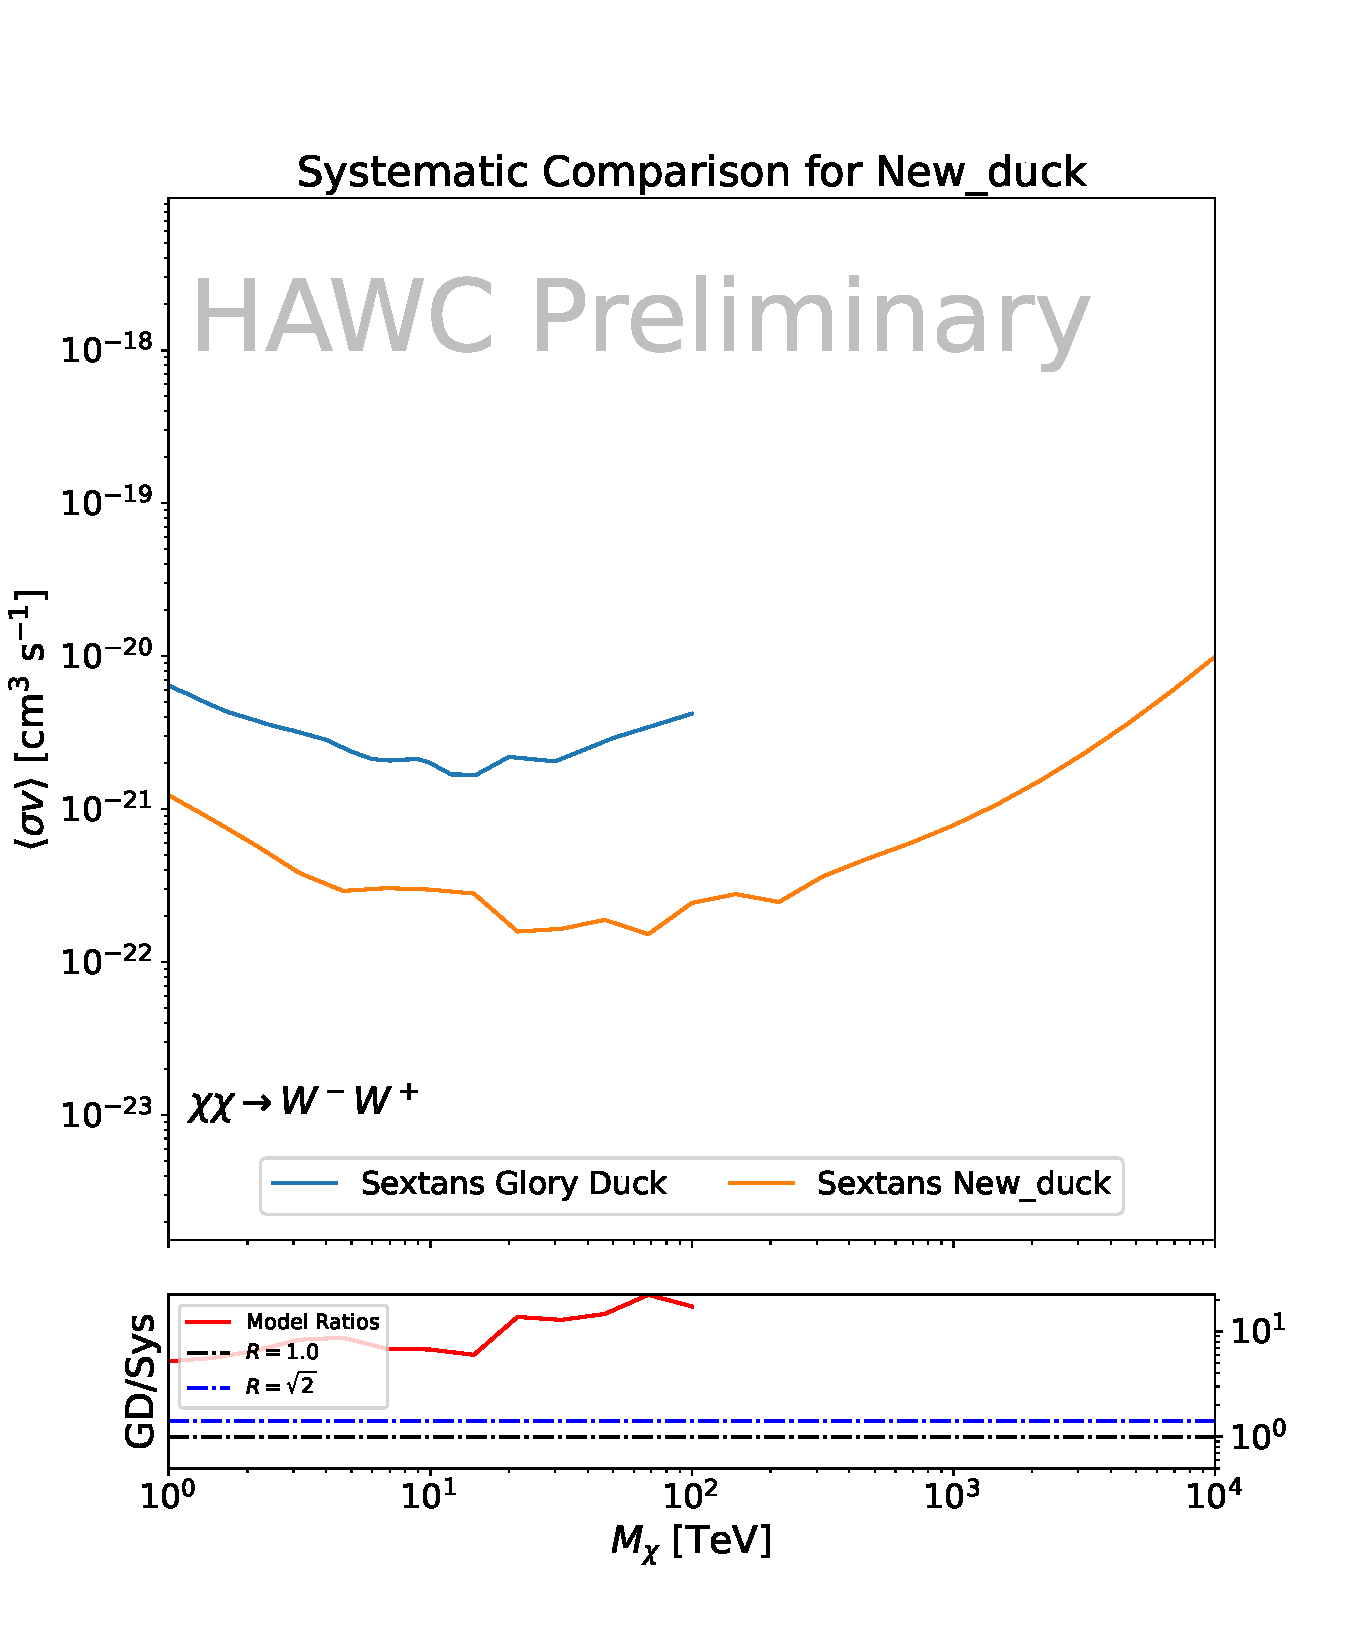
\includegraphics[scale=0.225]{figures/mtd_hawc_dm/systematics/Systematic_GD_New_duck_Sextans_ww.pdf}
    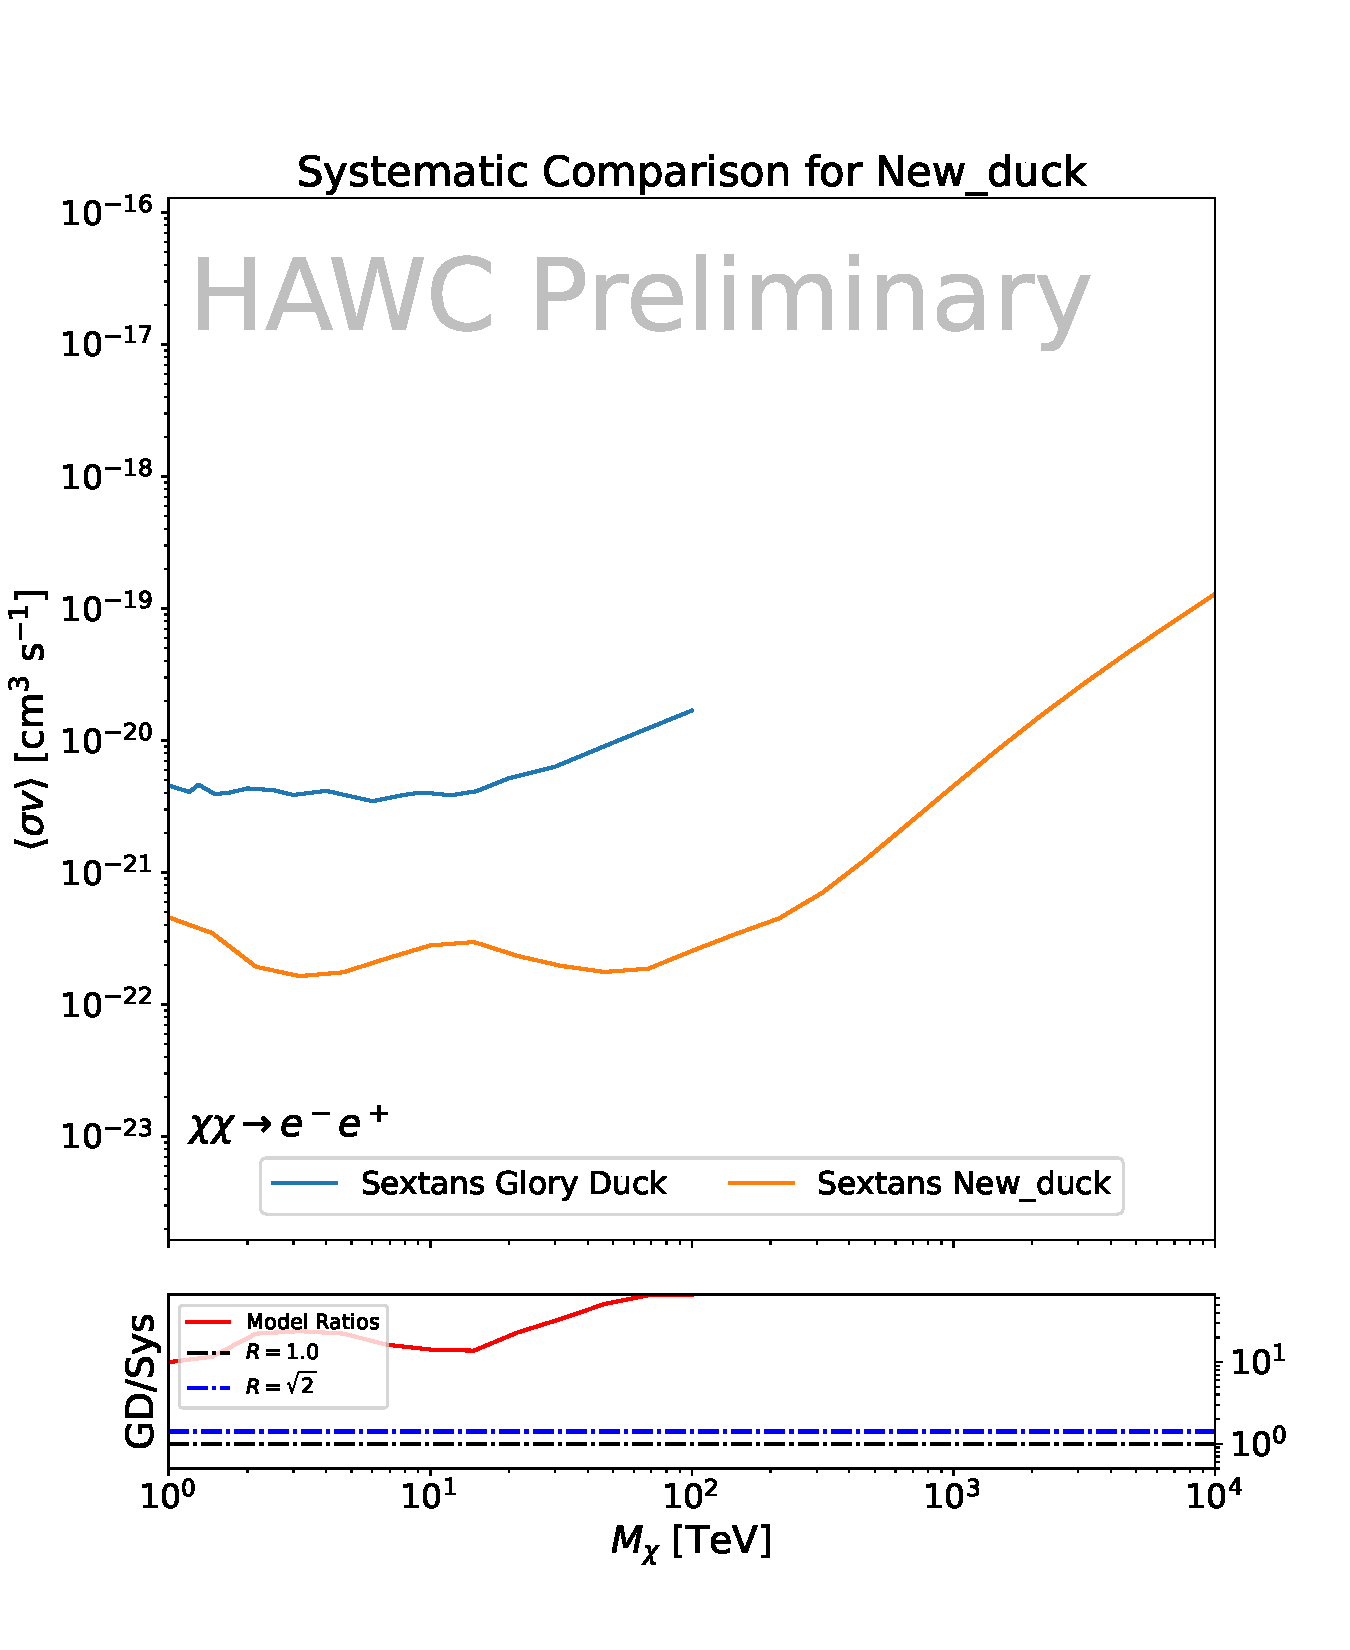
\includegraphics[scale=0.225]{figures/mtd_hawc_dm/systematics/Systematic_GD_New_duck_Sextans_ee.pdf}
    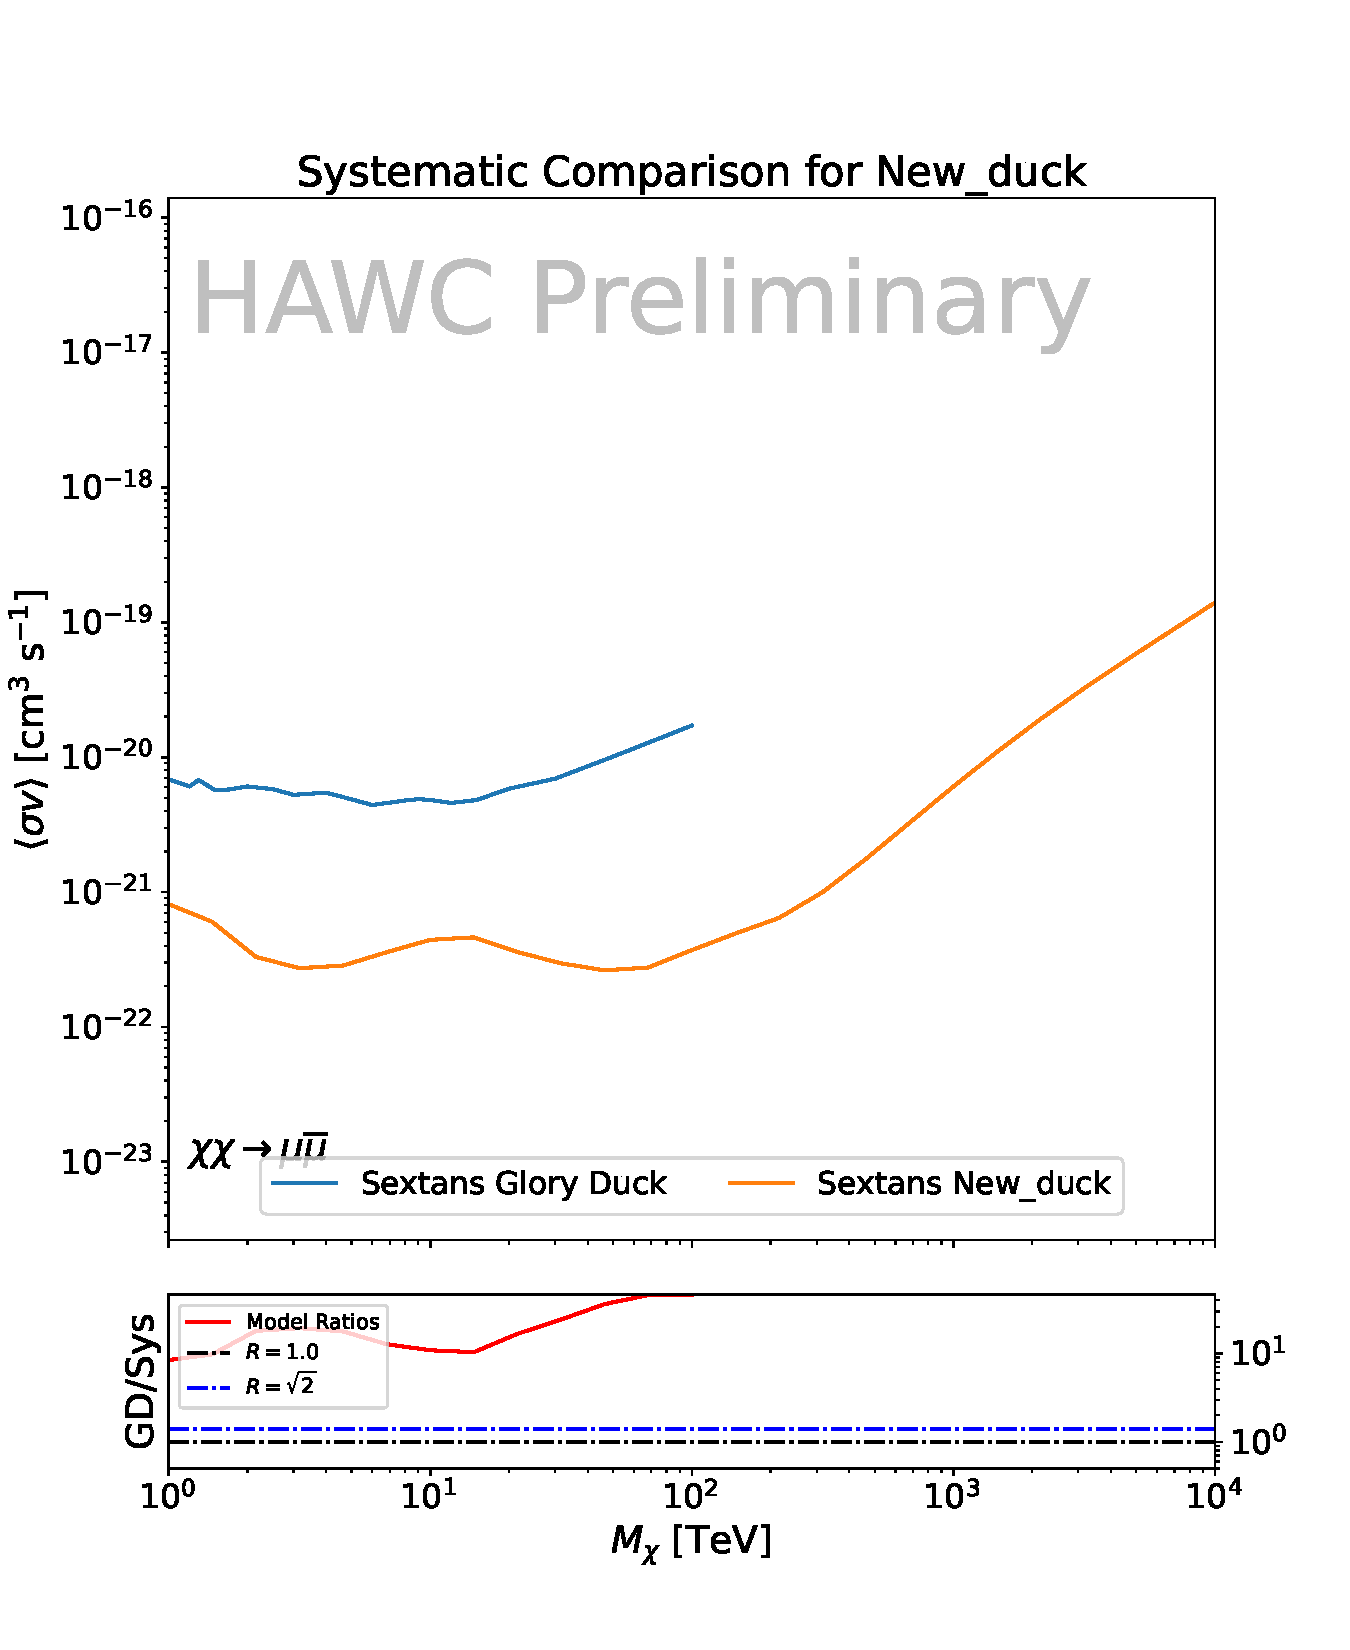
\includegraphics[scale=0.225]{figures/mtd_hawc_dm/systematics/Systematic_GD_New_duck_Sextans_mumu.pdf}
    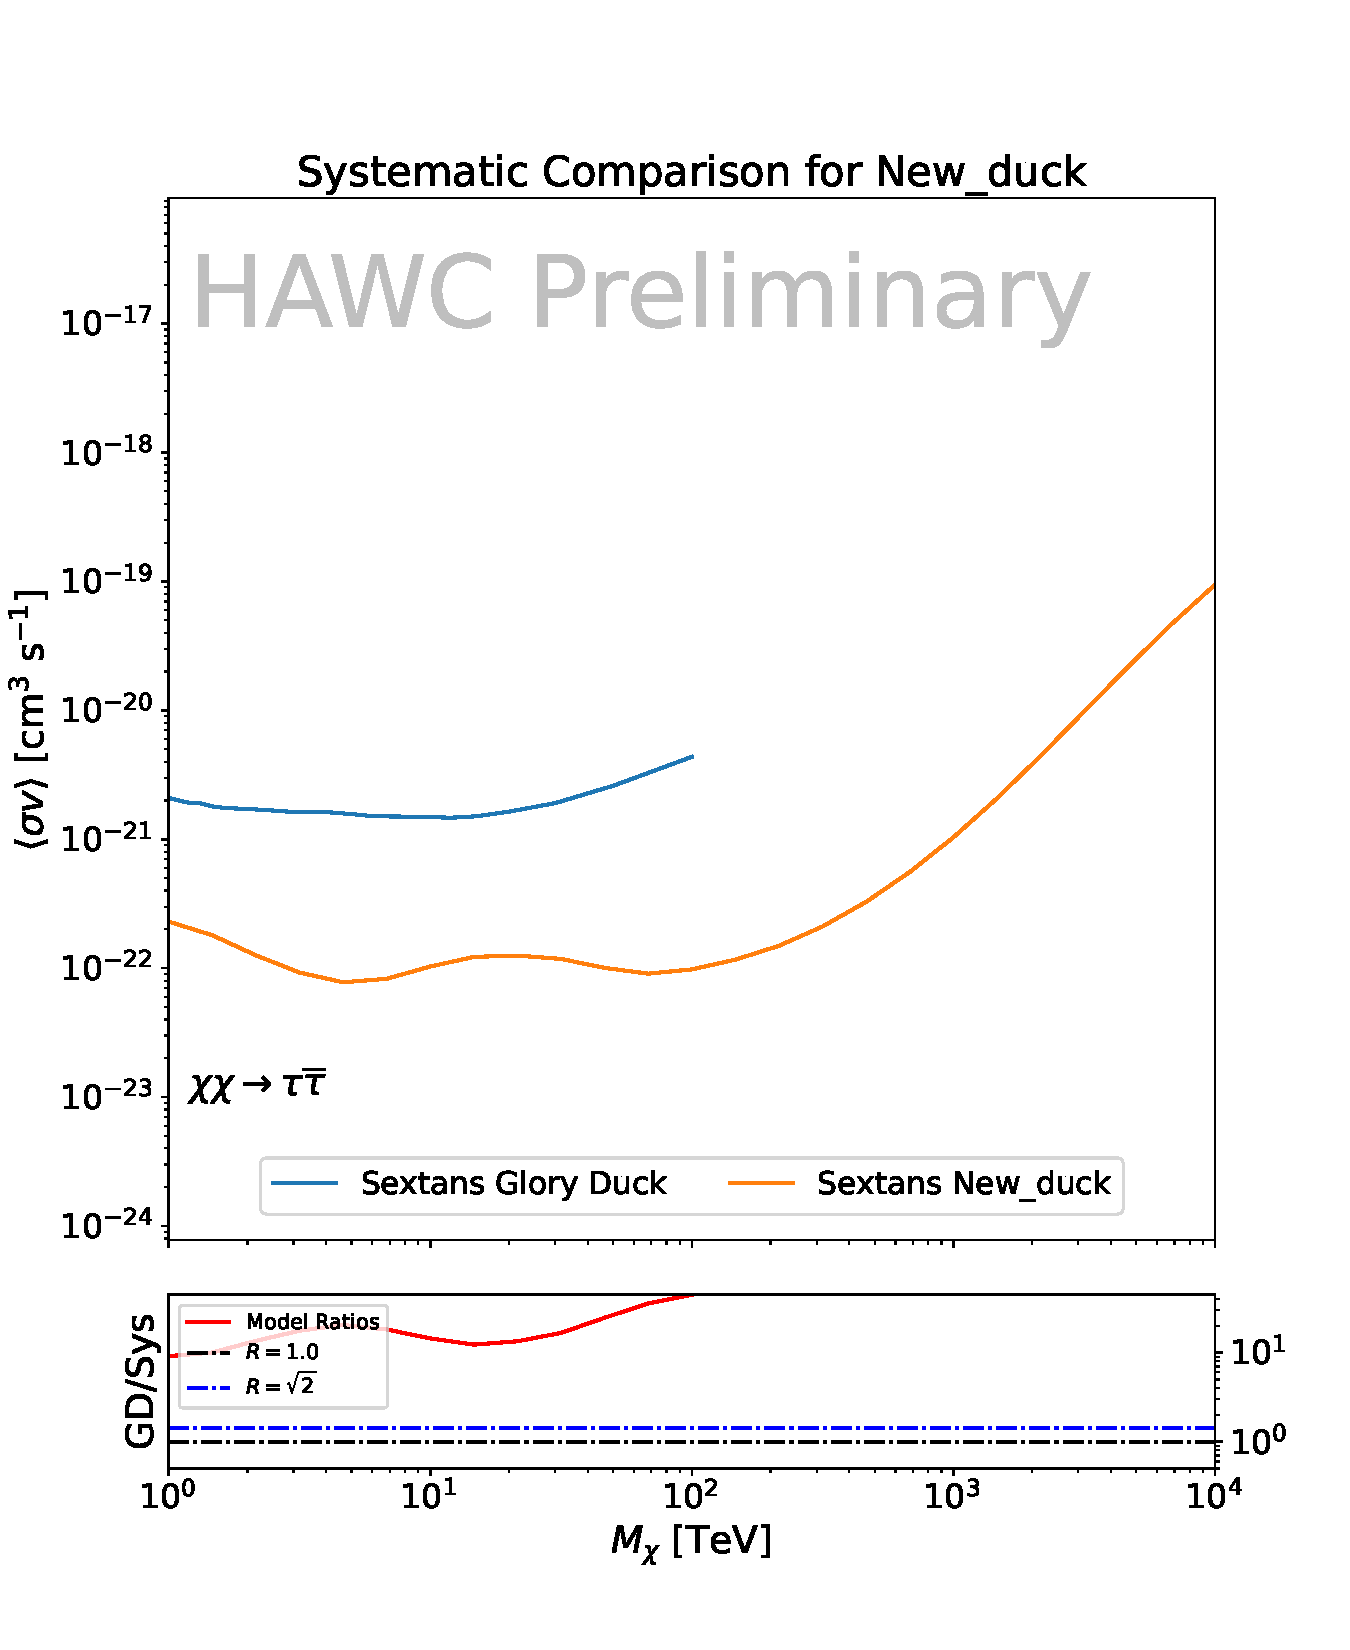
\includegraphics[scale=0.225]{figures/mtd_hawc_dm/systematics/Systematic_GD_New_duck_Sextans_tautau.pdf}
    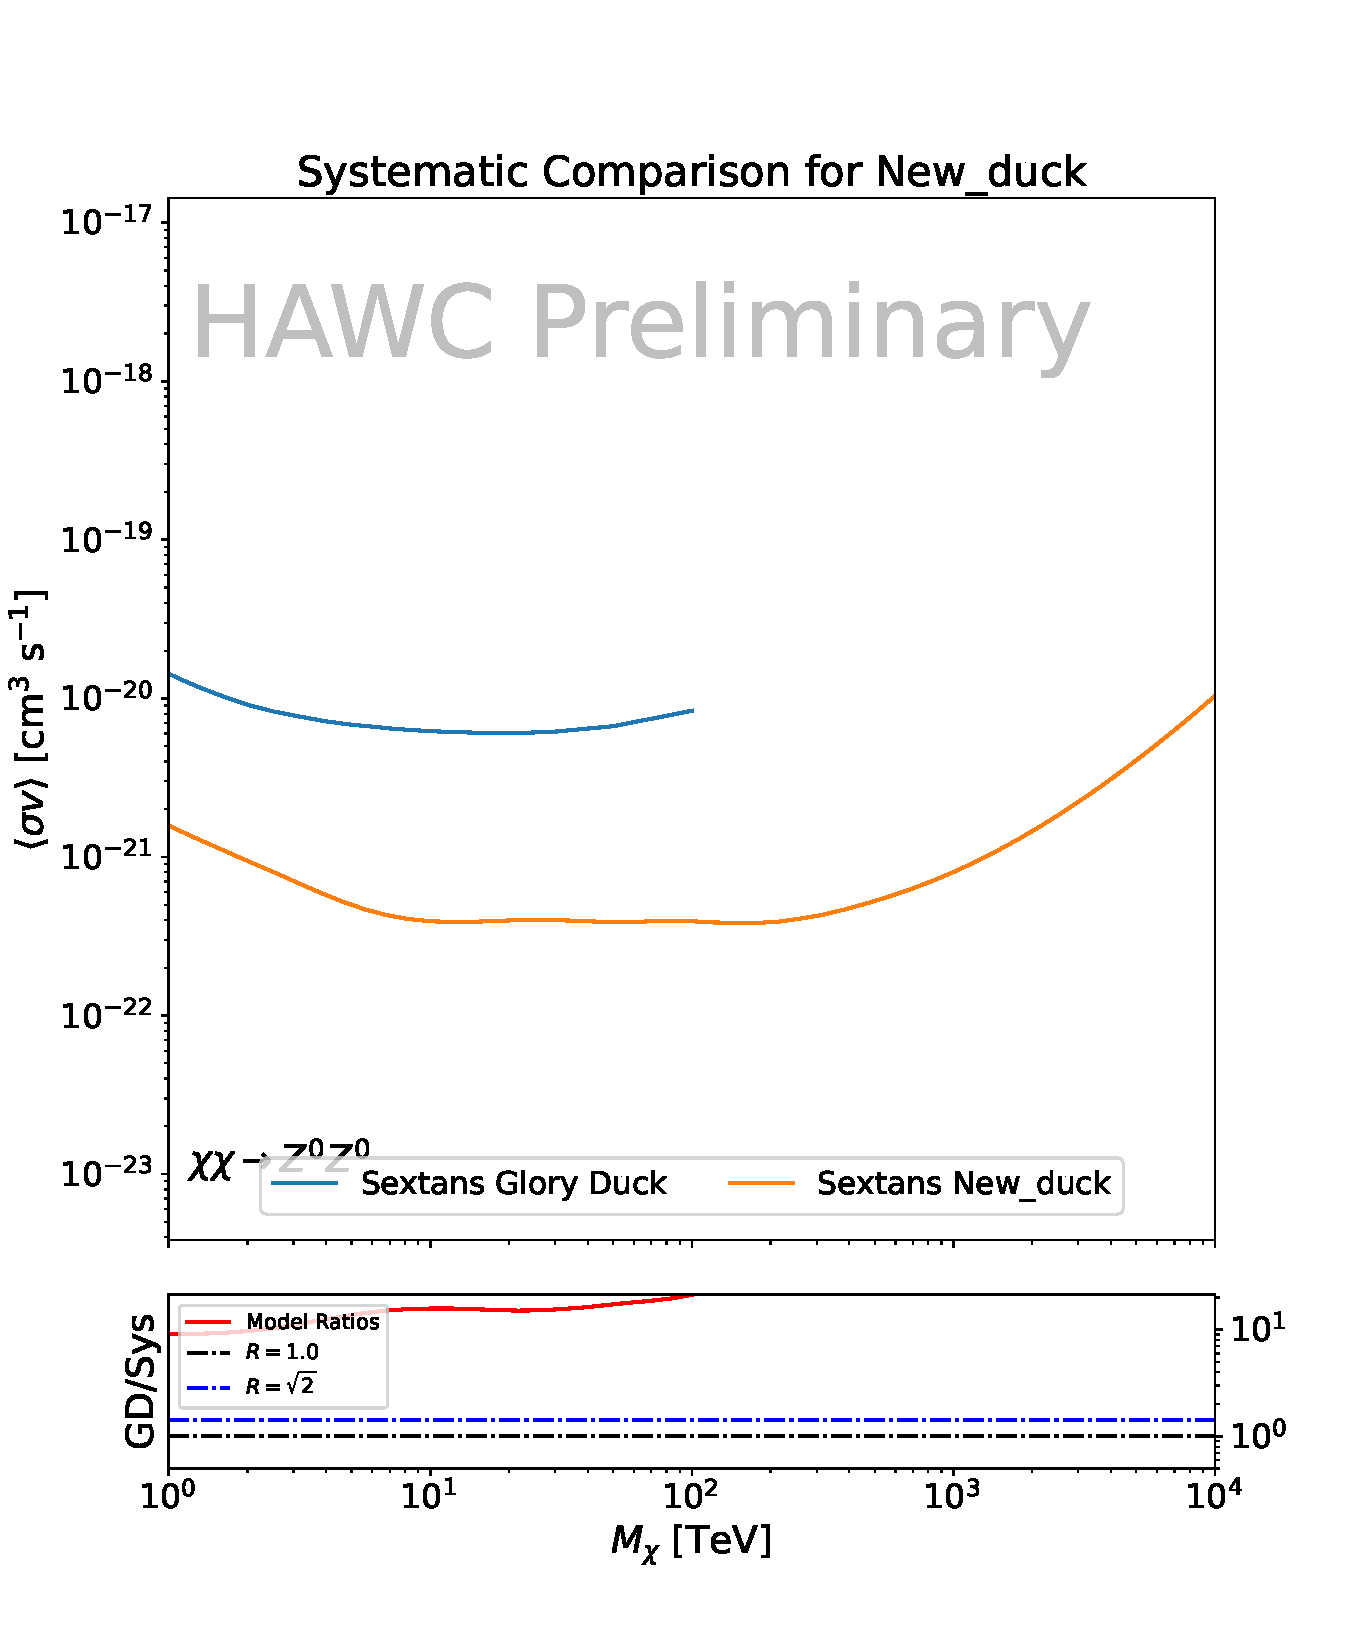
\includegraphics[scale=0.225]{figures/mtd_hawc_dm/systematics/Systematic_GD_New_duck_Sextans_zz.pdf}
    }
    \caption{Same as \cref{fig:mtd_compare_ComaB} but for Sextans.}
\label{fig:mtd_compare_Sextans}
\end{figure}